% options:
% thesis=B bachelor's thesis
% thesis=M master's thesis
% czech thesis in Czech language
% slovak thesis in Slovak language
% english thesis in English language
% hidelinks remove colour boxes around hyperlinks

\documentclass[thesis=M,czech]{FITthesis}[2012/06/26]

\usepackage[utf8]{inputenc} % LaTeX source encoded as UTF-8

%\usepackage{color}
\usepackage{graphicx} %graphics files inclusion
\usepackage{amsmath} %advanced maths
\usepackage{amssymb} %additional math symbols
\usepackage{listings}
%\usepackage[x11names]{xcolor}

\usepackage{caption}

%\usepackage{graphicx} %graphics files inclusion
% \usepackage{amsmath} %advanced maths
% \usepackage{amssymb} %additional math symbols
\usepackage{wrapfig}
\usepackage{tabularx}
%\usepackage{float}
%\restylefloat{table}

\usepackage{dirtree} %directory tree visualisation

%\usepackage{xcolor}
%\usepackage{color}
%%\usepackage{listings}

%\definecolor{dkgreen}{rgb}{0,0.6,0}
%\definecolor{gray}{rgb}{0.5,0.5,0.5}
%\definecolor{mauve}{rgb}{0.58,0,0.82}

\lstset{frame=tb,
  language=SQL,
  aboveskip=3mm,
  belowskip=3mm,
  showstringspaces=false,
  columns=flexible,
  basicstyle={\small\ttfamily},
  numbers=none,
%  numberstyle=\tiny\color{gray},
 % keywordstyle=\color{blue},
%  commentstyle=\color{dkgreen},
 % stringstyle=\color{mauve},
  breaklines=true,
  breakatwhitespace=true
  tabsize=3
}

% % list of acronyms
% \usepackage[acronym,nonumberlist,toc,numberedsection=autolabel]{glossaries}
% \iflanguage{czech}{\renewcommand*{\acronymname}{Seznam pou{\v z}it{\' y}ch zkratek}}{}
% \makeglossaries

\newcommand{\tg}{\mathop{\mathrm{tg}}} %cesky tangens
\newcommand{\cotg}{\mathop{\mathrm{cotg}}} %cesky cotangens

% % % % % % % % % % % % % % % % % % % % % % % % % % % % % % 
% ODTUD DAL VSE ZMENTE
% % % % % % % % % % % % % % % % % % % % % % % % % % % % % % 

\department{Katedra \ldots (Softwarového inženýrství)}
\title{
}
\authorGN{Dominik} %(křestní) jméno (jména) autora
\authorFN{Veselý} %příjmení autora
\authorWithDegrees{Bc. Dominik Veselý} %jméno autora včetně současných akademických titulů
\supervisor{Ing. Michal Valenta, PhD}
\acknowledgements{Chtěl bych poděkovat vedoucímu práce za podnětné, připomínky při tvorbě této práce. Dále bych chtěl poděkovat rodičům za podporu po celou dobu studia.}
\abstractCS{Tato práce shrnuje a definuje celý koncept BigData a jeho historii. Zabývá se také popisem technik, které jsou s tímto konceptem svázány, včetně vývoje pohledu na CAP theorém, který je nejznámějším theorémem spojeným s moderními distribuovanými systémy. V další části se práce zaměřuje na popis opensource technologií a to zejména Apache BigData platform. Největší důraz je kladen na NoSQL databázi Cassandru, která je v této práci stěžejní. Poslední část se zabývá reálnými případy užití Cassandry a přidružených technologií v praxi a popisem tvorby některých vybraných případů, které poslouží v rámci výuky v nově připravovaném předmětu. }
\abstractEN{This thesis sums up the whole concept of BigData and its history. It also describes techniques tightly related with this concept including evolution of how engineers look on CAP theorem which happens to be one of the biggest rules in modern distributed computing. In the next part thesis focus on opensource software from Apache BigData platform. It looks under the hood of NoSQL database Cassandra which is primary software for this thesis. Last part describes real use cases of Cassandra and related technologies in real world examples and description creation of certain use cases whose will be used in newly prepared course. }
\placeForDeclarationOfAuthenticity{V~Praze}
\declarationOfAuthenticityOption{4} %volba Prohlášení (číslo 1-6)
\keywordsCS{BigData, MapReduce, NoSQL, Cassandra, Sparse Collumn Database}
\keywordsEN{BigData, MapReduce, NoSQL, Cassandra, Sparse Collumn Database}


\begin{document}
	
% \newacronym{CVUT}{{\v C}VUT}{{\v C}esk{\' e} vysok{\' e} u{\v c}en{\' i} technick{\' e} v Praze}
% \newacronym{FIT}{FIT}{Fakulta informa{\v c}n{\' i}ch technologi{\' i}}

\begin{introduction}

Pro výběr tématu mé závěrečné práce mě motivovalo hned několik věcí. BigData jsou moderním trendem a technologií, která v současné době hýbe IT světem. Na druhou stranu je nutno říci, že je tento pojem značně zprofanovaný jeho až příliš častým využitím v marketingu konkrétních produktů. Mou první motivací tak bylo přinést ucelený a objektivní pohled na to, co to BigData jsou a naopak jasně vyčlenit, co nejsou tak, aby si čtenář dokázal po přečtení práce pod tímto pojmem jasně představit konkrétní technologie, metody a možnosti využití. 

Jak již bylo zmíněno, BigData jsou ve světě poměrně novým trendem. Další motivací tak pro mě bylo naučit se s něčím novým a zajímavým, s něčím s čím se mnoho lidí ještě nezabývá. Po oslovení vedoucího práce a po společné debatě nad možností využití tohoto tématu jako mé závěrečné práce, jsme došli k několika jasným cílům, které by tato práce měla naplnit. 

\subsection{Zmapování situace kolem BigData}
Jak již bylo zmíněno, jedním z cílů je poodhalit problematiku BigData jako takovou, k čemuž je nutné provést zmapování současného stavu v této oblasti. Zjistit nejčastější případy využití v akademické sféře nebo průmyslu, zmapovat aktuálně používané technologie a zároveň prozkoumat všechny přidružené technologie. 

\subsection{Využití zkušeností a znalostí a jejich rozvoj}
S NoSQL databázemi jsem měl předchozí zkušenosti, které jsem chtěl zužitkovat a prostřednictvím této práce navíc posunout mé znalosti dál. V rámci přípravy této práce jsem se zúčastnil Cassandra Summitu 2013 v Londýně, kde jsem rovněž absolvoval Cassandra Developer Training a získal jsem oficiální certifikát na vývoj s databází Cassandra přímo od jejího výrobce firmy Datastax. Vzhledem k tomu, že se práce zabývá především Cassandrou, považuji toto školení za velký úspěch a samotný summit za velice přínosný především pro kapitolu věnovanou případům využití.

\subsection{Příprava nového předmětu na ČVUT}
BigData jsou moderní technologickou i vědní disciplínou a Fakulta informačních technologií (konkrétně Katedra softwarového inženýrství) projevila zájem o vytvoření nového předmětu, který by se po praktické stránce věnoval BigData a databázovým systémům. Pod dohledem vedoucího katedry a vedoucího práce Ing. Michala Valenty, PhD tento předmět připravuje Ing. Josef Gattermayer a tato práce by měla sloužit jako pomůcka pro přípravu tohoto předmětu a to především po stránce praktických příkladů, které z ní vzejdou a poslouží jako náměty na možná témata cvičení, či rovnou jako hotová řešení. 

\subsection{}
V následujících kapitolách se postupně věnuji všem třem výše vytyčeným cílům, které se prolínají se zadáním této práce. 




\end{introduction}


\chapter{Co jsou to BigData}



Popsat termín BigData není úplně snadné, a to hned z~několika důvodů. Především proto, že neexistuje žádná přesná definice tohoto pojmu. Tento termín je stejně jako obor, kterého se týká, velice dynamický a rychle se mění. K~obtížnější definici pojmu přispívá také fakt, že se hojně používá v~marketingové komunikaci jako tzv. \uv{buzzword} za účelem vzbudit zájem čtenáře/posluchače, přestože může být použit v~nesprávném kontextu.

Termín BigData označuje manipulaci s~datasety tak velkými, že je nemožné nebo velice obtížné s~nimi manipulovat za pomocí tradičních nástrojů a databází (převážně relačních). Pod pojmem manipulace s~datasety myslíme:

\begin{itemize}
  \item Sběr
  \item Organizace
  \item Ukládání
 \item Prohledávání
 \item Sdílení
 \item Analýza
 \item Vizualizace
\end{itemize}

Nalezení této hranice či její přesná definice je komplikovanější problém mimo rozsah této práce. Na toto téma již bylo publikováno mnoho jiných prací. Jak jsem zmínil již v~úvodu, práce se dále také nezabývá porovnáním BigData a klasických relačních databází. 

V~této kapitole se pokusím obecně přiblížit, co to tedy BigData jsou, jak se liší a důvod vzniku tohoto odvětví.


\section{Trend velkých datasetů}
Jak jsem již naznačil, BigData se věnují zpracování velkých datasetů. Trend upřednostňování velkých datasetů oproti několika menším, které v~součtu mají stejný objem a nesou stejné množství informace, začal vzhledem k~jednoduššímu hledání a objevení i zdánlivě neexistujících korelací, projevení obchodních trendů a vyhodnocování dat v~reálném nebo skoro reálném čase.

\section{3V}
Jak naznačil předchozí odstavec, BigData nejsou pouze o~objemu zpracovávaných dat, jak by se na první pohled mohlo zdát. Jedná se o~komplexnější kategorizaci, kde hrají roli i ostatní charakteristiky, které se v~literatuře značí zkratkou 3V, odvozenou od počátečních písmen těchto kategorií v~anglickém jazyce.

\begin{figure}[h]
\centering
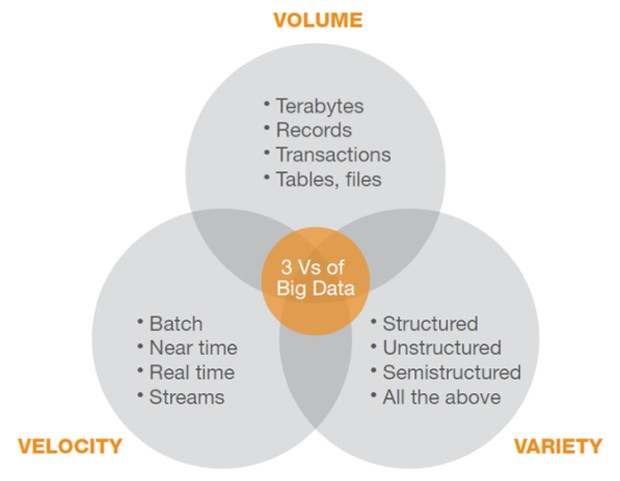
\includegraphics[scale=0.6]{images/3v}
\caption{Schéma popisující 3V pomocí množinových diagramů \cite{3vimg}}
\label{fig:3v}

\end{figure}

\subsection[3v-volume]{Obsah (Volume)}
Data se dnes zdaleka nevyskytují jen v~textové podobě, můžeme je uchovávat formou hudby, obrázku či videa. Vzhledem k~tomuto faktu čelíme exponenciálnímu nárůstu množství uchovávaných dat a není výjimečné, aby enterprise systémy uchovávaly terabyty nebo petabyty dat. Data tedy tvoří množství informací, které je dost často vyhodnocováno z~různých úhlů a následně uloženo a znovu vyhodnocováno, a přestože původní data zůstala nezměněna, díky reevaluaci nám jejich množství roste závratným způsobem. Tímto způsobem může být na objem nahlíženo jako na jednu z~charakteristik BigData.

\subsection{Rychlost (Velocity)}
Na rychlost můžeme nahlížet hned ze dvou pohledů. Prvním pohled vyjadřuje rychlost, jakou nám data přibývají a jak aktuální pro nás jsou. Například historie vývoje měnového kurzu je informace, jejíž včerejší hodnota je naprosto nevypovídající a mění se s~každou minutou. Změnila se i rychlost, jakou noviny a televizní stanice získávají informace skrze sociální sítě. Objem dat tedy roste rychle a aktuálnost informací se rapidně zkrátila. Druhý pohled na tuto charakteristiku se zabývá rychlostí, jakou data potřebujeme zpracovávat. Jsou informace, které k~nám proudí velice často (například každou minutu), ale jejich vyhodnocení dává smysl ku příkladu jen jednou za 24 hodin. Ovšem jsou také data, které potřebujeme zpracovávat v~reálném čase, tak, jak k~nám proudí. Dobrým příkladem takových dat mohou být akutální informace z~meteorologické stanice. 
Rychlost, v~jaké jsou dnes data zpracovávána, se mnohonásobně zmenšila a tedy nejen objem dat, ale i rychlost zpracování reprezentuje samotná BigData.

\subsection{Různorodost (Variety)}
Jak je z~Obrázku ~\ref{fig:3v} patrné, různorodost dat znamená jejich strukturovanost/nestrukturovanost. Již bylo zmíněno, že data mohou mít mnoho podob. Ale i data ve stejné podobě (například textové), mohou být jinak strukturována a tomuto faktu je potřeba se přizpůsobit a uchovávat a zpracovávat data v~jiných formátech.
Různorodost a adaptabilita jsou tedy posledními charakteristikami BigData.

\section{BigData zjednodušeně}
Předcházející řádky by měly sloužit jako shrnutí a lehký úvod do problematiky BigData. Dalo by se vlastně také říci, že BigData nejsou jen o~velkém množství dat, ale je to celý koncept uchovávání a možností nových náhledů na stávající data, ale také návod, jak zachytit a zpracovat budoucí data. Další odstavce budou věnovány historii tohoto konceptu, ale také nejtypičtějších odvětví, kde se s~ním můžeme setkat. 

\section{Historie}

Již od počátků počítačové éry bylo potřeba data analyzovat. \cite{history} S~rychle se zvyšující dostupností moderních technologií a jejich obecnému přijetí ve společnosti, se posouvaly hranice této potřeby od vládních organizací až po současnost, kdy obrovské množství informací a jejích analýzu potřebují i malé podniky.

\subsection{30. a 40. léta}
V~této době se používaly první počítačové simulace. Prim hrálo především válečné odvětví, kde například vědci z~projektu Manhattan pomocí počítačových simulací simulovali dopad a následný zničující efekt jaderné bomby.

\subsection{50. a 60. léta}
V~tomto období se počítače (a s~nimi také zpracování a analýza dat) rozšířily do velkých korporací a výzkumných laboratoří. Počítač ENIAC například generoval první modely pro předpověď počasí. Analytici také vyřešili první problém nejkratší cesty a mnoho dalších, viz. také \cite{history}.

\subsection{70. až 90. léta}
V~této době se analytická činnost rozšířila o~středně velké podniky a technologické startupy. Objevují se také dnes již dobře známé případy užití. Dobrým příkladem takových případů je třeba první predikční model na pokles a růst akcií. Dále také stojí za zmínku první komerční nástroj pro modelově řízené rozhodování. Důležitým milníkem je rovněž vznik společností, jako je Ebay a Amazon. Bitva o~personalizaci online nákupů právě začala! Google implementuje první vyhledávací algoritmus, který zvyšuje relevanci výsledků.

\subsection{2000 až součanost}
V~tomto období se analytika rozšířila až na oblast malých podniku a analytických expertů (jednotlivců). Začíná mít obrovský dopad na život každého z~nás. Samozřejmostí začínají být dynamické změny cen zboží, doporučování produktů, hudby a filmů nebo řízení dopravy. Rozvíjejí se obory, jako je analýza a procesování přirozeného jazyka z~novin, e-mailů nebo sociálních sítí. Příchodu BigData, vzhledem k~levné dostupnosti výpočetního výkonu a rychlosti zpracování dat, již nic nestojí v~cestě.

\subsection{Budoucnost}
Předpokládá se, že v~budoucnu bude analytická činnost řídit každodenní rozhodování i na úrovni jednotlivců. V~běžném životě se přínos analýzy dat projeví například: Predikce v~policejní sféře a boji proti zločinu, výzkum ve zdravotnictví nebo kompletně personalizovaná zákaznická interakce i pro malé podniky a řetězce.

\section{Nástup sociálních sítí}
BigData zažila obrovský nástup také díky příchodu a masivnímu rozšíření sociálních sítí, a to hned ze dvou důvodů. Prvním důvodem je, že nástup sociálních sítí přilákal tisíce výzkumníků, kteří začali sbírat data z~Facebooku a Twitteru. Tito výzkumníci následně hledali různá spojení mezi zprávami a účty, z~kterých poté vyvozovali závěry ohledně těchto sociálních sítí. Další možností, k~čemu vytěžená data používali, bylo vytváření tzv. sociálních grafů. Historicky sbírali antropologové a sociologové data o~lidských vztazích skrze dotazníky, rozhovory, pozorování a experimenty. Dolováním dat ze sociálních sítí, kde lidé sdílejí mnoho detailů ze svých životů, se jim otevřel nový kanál, kde mají všechny tyto informace jednoduše k~dostání a stačí je pouze analyzovat.

V oblasti sociálních sítí existují 2 konkrétní druhy, které jsou z hlediska konceptu BigData zajímavé: \uv{Artikulované sítě} a \uv{Behaviorální sítě}. První kategorie znázorňuje sítě, kde uživatelé zadávají svá přátelství a konexe skrze technické mechanismy jako například: telefonní seznamy, emaily, seznamy přátel z~jiných sití atd. Druhou kategorií jsou sítě odvozené od komunikačních vzorců. Do této skupiny spadají uživatelé, kteří si píšou zprávy nebo jsou označení na společných fotkách. Obě tyto skupiny mají pro výzkumníky velký význam, přestože jím nepřikládají takovou váhu jako reálným osobním vztahům. \cite{social} 

Druhým důležitým aspektem, proč jsou sociální sítě pro BigData důležité, je fakt, že tyto sítě samy potřebují někde svá data uchovávat a zpracovávat. Technologické týmy stojící za těmito službami se tak ve značné míře podílejí jako kolaborátoři na BigData projektech či dokonce vytvářejí a následně uvolňují svoje technologie k~užití pro širokou veřejnost. Pro komunitu jsou důležité i přednášky a prezentované poznatky od těchto datových gigantů, kteří prozkoumávají a prolamují lidstvu dosud známe bariéry a umožňují tím využívání technologických pokroků i jiným subjektům. 

Sociální sítě samozřejmě nejsou jediným průkopníkem na poli BigData. Internetoví giganti jako Google, Amazon a Yahoo přispívají neméně výrazným dílem. Na sociálních sítích je však zajímavé to, že jejich data jdou do jisté míry jednoduše dolovat, díky čemuž vzniklo mnoho spolčeností, které se začaly jejich analýzou a sběrem zabývat a způsobily tím popularizaci spojení BigData se sociálními sítěmi. 


\section{Odvětví}

Jak již bylo zmíněno v~předchozí sekci, v~dnešní době můžeme na BigData narazit kdekoliv. Zde bych chtěl poukázat na široké spektrum využití napříč různými činnostmi, kterými se lidstvo zaobírá.\cite{sektory}

\subsection{Maloobchod}
Péče o~zákazníka a samozřejmě také zvýšení zisku jsou hlavními motivy pro zpracovávání a analýzu dat. Na základě chování uživatelů (aktivita na webu, zákaznická karta, anonymní zákazníci) můžeme předpovídat chování zákazníka v~každém stádiu nákupu. Toto chování lze navázat také na podniková data a hledat korelace pomocí Map Reduce mechanismů. Největším průkopníkem spojování BigData a maloobchodu je bezesporu řetězec Tesco se svou věrnostní kartou ClubCard. Na základě zákazníkovy nákupní historie sestavují žebříček produktů k~doporučení či dokonce dokáží odhadnout období těhotenství svých zákaznic.\cite{tesco}

\subsection{Věda a výzkum}

Není žádným překvapením, že ve vědě a výzkumu se využívají BigData na uchovávání výsledků z~měření či pro hledání korelací v~naměřených hodnotách. Držitel Nobelovy ceny Peter Higgs používal NoSQL databázový systém Cassandra na zpracování svých dat, díky nímž prokázal existenci tzv. Higgsova Bosonu \cite{higgs}.

\subsection{Meteorologie}
Díky sběru a vyhodnocování dat z~meteorologických stanic se podařilo vytvořit mnohem spolehlivější a přesnější modely pro předpovědi počasí, a to jak dlouhodobých, tak také krátkodobých. 

\subsection{Finance}
Ve finančním sektoru je způsobů využití hned několik. Například již výše zmíněné doporučování produktů dle historie transakcí a sběru  osobních dat. Banky a jiné finanční instituce podobným způsobem nabízejí zákazníkům vhodné finanční produkty, jako jsou například hypotéky. Mnohem zajímavějším případem využití BigData je detekce podvodů, kdy jsou banky na základě analýzy všech transakcí schopny hledat vzory podvodných chování a vyhodnotit určité transakce jako podezřelé a tím tak chránit své klienty nebo samy sebe.

\subsection{Webová optimalizace}
Na základě ukládání a následného zpracování veškerého chování uživatele na stránce mohou firmy optimalizovat webové stránky a jejich obsah či ho případně restrukturalizovat. Po vyhodnocení chování konkrétních uživatelů je možné jim obsah stránky automaticky personifikovat a podsouvat tak uživatelům pro ně zajímavé věci, aniž by se k~nim museli složitě proklikávat.

\subsection{BioInformatika}
V~bioinformatice se BigData využívají například k~mapování genomů nebo k~sekvenční analýze. Tyto informace pomáhají k~lepšímu pochopení DNA a také k~prevenci genetických poruch a vrozených nemocí či k~usnadnění jejich léčby. \cite{industries} 

\section{Dnešní možnosti}
V~dnešní době existují v~podstatě 3 možnosti jak začít s~BigData. 

\subsection{Specializované firmy a hotová řešení}
Na internetu nalezneme několik firem zabývajících se analýzou vašich dat, kde veškerá analýza a vizualizace probíhá v~softwaru třetí strany. Mezi nejznámější patří společnost Good Data \cite{gooddata}. Tyto firmy se však specializují na zpracování firemních dat a vizualizaci v~jejich vlastních BI nástrojích.

\subsection{Hotová enterprise řešení}
Další možností je vybrat nějaké komplexní řešení od firem zabývajících se platformou BigData, které vám dodají software pro ukládání, analýzu a vizualizaci vašich dat. Programování komponent či jejich konfigurace je v~režii zákazníka a tyto firmy poskytují licence, školení a technickou podporu. Tuto možnost poskytuje například IBM.

\subsection{Open Source a řešení z~něj vycházející} 
Poslední možností je použití Open Source nástrojů, které umožní ukládat, analyzovat a vizualizovat data. Toto je cesta, kterou jsem se vydal v~rámci této práce a budu se jí tak nadále věnovat. Drobnou nadstavbou těchto řešení mohou být firmy nabízející komerční balíčky těchto Open Source řešení. Jedná se o~velice populární přístup v~případech, kdy je potřeba zkombinovat několik nástrojů dohromady. Jejich konfigurace bývá velice obtížná, a proto tyto komerční balíčky nabízí již nakonfigurovaná hotová řešení většinou i s~drobnou nadstavbou, která umožňuje provádět některé nadstandardní procesy a činnosti. 



%mozna jen podsekce bigdata%
\chapter{BigData techniky}



Abychom mohli hovořit o konkrétních technologicích, musíme nejdříve definovat základní stavební technologické kameny, o které se BigData opírají. Jedná se o technologie a paradigmata vyvinutá technologickými giganty, kteří jako první naráželi na technologické hranice a posouvali je dál a tak se postupně rodily tyto technologie a paradigmata. Jejich pořadí se odvýjí od logické posloupnosti tak, jak spolu souvisí a navazují na sebe.    

\section{Distribuované systémy}
Distribuované systémy, jsou tématem, které zasahuje samozřejmě mnohem dále, než jen do kategorie big data. Pro zjednodušení následujících řádků, zavedeme následující rozdělení. Distribuované systémy rozdělíme na systémy s distribuovaným výpočetním výkonem, systémy s distribuovaným úložištěm a nebo kombinace obojího. 

Distribuovaný výpočetní výkon, je takový systém, kde se výpočet jedné úlohy rozloží na více počítačů. Paralelní výpočety jsou známé z oblasti informačních technologií, již mnoho let a používají se nejčastěji k vědeckým výpočtům, paralelní kompilaci zdrojových kódů a nebo k jiným operacím, které by na jednom počítači trvaly příliš dlouho. 

Distribuované úložistě je jednoduše představitelné a důvodů mít data na více místěch je hned několik.
\begin{itemize}
\item Záloha - i ze sféry osobních počítačů známé trend kde máme data zálohovaná na více fyzických zařízeních, abychom předešli jejich ztrátě, v případě technické poruchy na daném zařízení. 

\item Nedostatek kapacity - Ze sféry osobních počítačů známe, že uživatelé, méně potřebné soubory ukládají na externí periferie, protože kapacita disků v osobních počítačích je zpravidla kolem pár TB.

\item Dostupnost - Pokud chce uživatel mít přístup k jednomu souboru z domácího i pracovního počítače, musí soubor mít fyzicky na těchto dvou počítačích, nebo využít nějaký software na sdílení souborů. 

\end{itemize}

Kombinovaný přístup je zřejmy a tedy, že se používá jak výpočetní výkon jednotlivých počítačů v systému, tak jejich úložný prostor. 

Big Data využívá všechny tyto přístupy, je zřejmé že obrovské množství dat, o kterém jsme mluvili v úvodu se lépe zpracovává na více počítačích. Stejně tak je logické, že pokud budeme bavit o množství dat, tak velké množství dat, uložíme na více počítačů, stejně tak pokud data chceme zálohovat. 

Ne vždy však využíváme kombinovaný přístup, je totiž velmi časté, že si firmy staví obrovské počítačové farmy, které slouží pouze jako datové sklady a datová centra. Vždy záleží na konkrétní situaci a způsobu využití. 


\section{CAP Theorem}
V roce 2000 při nástupu distribuovaných systémů vydal vědec Eric Brewer článek, popisucjíí tzv. CAP Theorem \cite{cap}, který se distribuovaných systémů přímo týká. Teorém říká, že distribuované systémy mají tyto 3 hlavní vlastnosti. 

\begin{itemize}
\item Konzistence (Consistency) - Vlastnost, která určuje, zda pro každý požadavek, vratí server správný výsledek. to znamena že odpověd je adekvátní vůči specifikaci požadované služby. Přesný význam konzistence se odvýjí od typu služby. V případě dat ji definujeme tak, že každý server má aktuální a stejná data.

\item Dostupnost (Availability) - Vlastnost která říka, že každý požadavek dostane odpověd. Rychlejší odpověd, je preferovanější oproti pomalejší, ale v kontextu teorému je důležité, že odpověd dorazí. V praxi však znamená, že velice opožděná odpověd je stejně spatná jako žádná odpověd a můžeme tuto vlastnost zjednodušit, že systém vždy musí být dostupný.

\item Tolerance výpadku (Partiotion tolerance) - Tato vlastnost jako jediná určuje chování podpůrného systému na kterém služba běží, namísto popisu chování služby samotné. Tato vlastnost říká, jestli během výpadku nějaké části systému, je systém schopný pokračovat a dále fungovat.

\end{itemize}


Brewer popisuje, že každý distribuovaný systém může splňovat nejvýše 2 z těchto 3 vlastností.

\subsection{CAP Theorem v roce 2012}
V roce 2012 napsal Brewer další článek \cite{cap2}, ve kterém popisuje stav jeho theorému po 12 letech. Vysvětluje, že již od začátku bylo označení \uv{pouze 2 ze 3} zavádějící a vágní, protože spoustu věcí příliš zjednodušovalo. Například u systému s velkou granularitou,  se mezi volbou C a A rozhoduje na několika úrovních a všechny vlastnosti mají spíše hodnoty v čase, než binární a také, že záleží na stavbě systému a jeho drobných nuancích. Také ale píše, že v důsledku theorém splnil svůj účel a otevřel tak systémévým návrhárům oči pri navrhování distribuovaných systémů a donutil je zamyslet se nad vyhodami a nevýhodami jednotlivých vlastnotí systému. 

V témže roce vyšel další zajímavý článek popisující aktuální stav CAP theorému \cite{cap3}. Popisuje převážně vztah
systémů k volbám CAP vlastnostní. 

\subsubsection{Nejlepší možná dostupnost}
Nejčastejší výběr je garantovaná konzistence s maximální možnou dostupností, pro většinu systémů je toto přirozenou volbou. Tedy, že za každou cenu, server vrací správnou odpověd a snaží se poté optimalizovat co největší dostupnost a nejrylechjší možnou odpověd vzhledem k síťovým podmínkám. Tento přístup dává největší smysl pokud jsou počítače ve stejném datacentru a běží na nich stejná služba. Typickým zástupcem je  \uv{lock service} a služba spravující metada pro nějaký distribuovaný systém s nízkou granularitou.

\subsubsection{Nejlepší možná konzistence} 
Druhou nejčastější skupinou jsou systémy, pro které je ztráta dostupnosti nemyslitelná a tudíž garantují dostupnost a snaží se o co nejvyšší úroveň konzistence. Tento postup nejlépe vyhovuje v případech kdy máme počítače distribuované napříč několika datacentry, v tomto případě může totiž dostupnost rapidně klesat s jakoukoliv chybou a proto je potřeba ji garantovat. V těchto případech tedy designéři obětují konzistenci, aby mohli garantovat dostatečně rychlou odpověd, přestože ta nemusí být vždy zcela správná. Ideálním příkladem jsou webové cache a obrázkové servery.

\subsubsection{Segmentovaná konzistence a dostupnost}
toto je nejzajímavější možnost a pro tuto práci je také nejdůležitější. Existují systémy, které nemají jednotné požadavky pro všechny aspekty služby. Některé vyžadují silnou konzistenci a některé vysokou dostupnost. Pro dodžení CAP theoremu se  jako nejpřirozenější možnost jeví rozdělit systém na několik jednotlivých komponent, které budou specificky nastaveny. tím tedy celý systém nezaručuje ani konzistenci, ani dostupnost, ale každá část systému postkytuje opravdu vlastnosti, které potřebuje. Segmentace může probíhat na několika možných úrovních. 

\begin{itemize}
\item \textbf{Rozdělení podle dat} - jiná data mohou vyžadovat jinou úroveň dostupnosti a konzistence.
\item \textbf{Rozdělení podle operací} - Operace pro zápis mohou mít jiné požadavky na konzistenci a dostupnost, než operace pro čtení.
\item \textbf{Rozdělení podle funkcí} - Některé služby mohou být rozděleny na podslužby a tedy pro každou takovouto službu můžeme mít vlastní úroveň konzistence a dostupnosti. 
\item \textbf{Rozdělení podle uživatelů} - Jedná se o rozdělení závislé převážně na geografické poloze uživatele, služba bude pro uživatele, který se nachází blízko může zaručit vysokou dostupnost a zároveň v rámci jeho blízkého data centra udržovat i konzistenci. 
\item \textbf{Rozdělení podle hierarchie} - Jedná se o systém ve kterém se na určitých úrovních kombinují výše popsané rozdělení.
 
\end{itemize}
\section{Distribuovaný file systém}

V předchozích sekcích jsme rozebrali distribuované systémy a jejich omezení. Zmínili jsme také, nutnost sdílet velké množství dat napříč několika počítači, které můžou být napříč různými datacentry. Tuto potřebu, tedy mít distribuovaný filesystém, měl i jeden z největších technologických gigantů, firma Google. V roce 2004, se Google rozhodl o jejich řešení podělit a vydal detailní článek \cite{gfs} popisující kompletní funkčnost a detaily celé infrasntruktury. Vysvětlení funkčnosti a  architektury je nad rámec této práce a navíc je vše dobře popsané v článku samotném, důelžité je však zmínit, že tento systém se stal inspirací a nastolil trend v tom, jak podobné systémy dnes vypadají a jaké mají vlastnosti. Na základě tohoto článku vznikl například opensource klon MooseFS.

\begin{figure}[h]
\centering
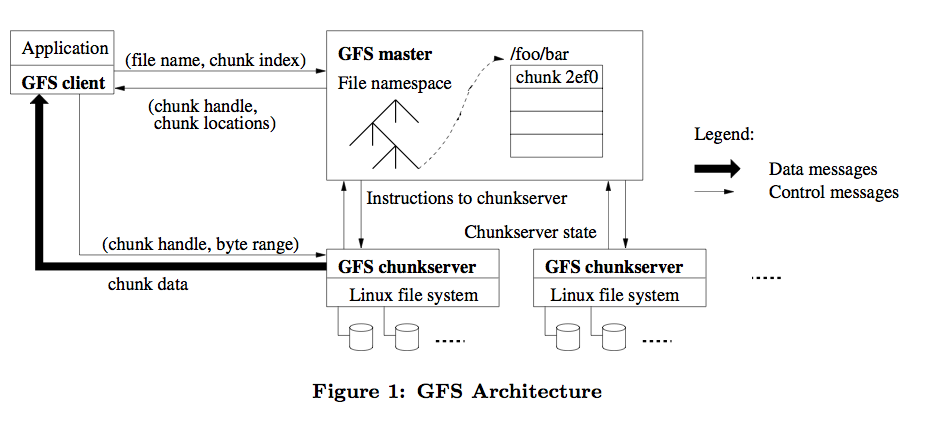
\includegraphics[scale=0.5]{images/gfs}
\caption{Architektura Google File System \cite{gfs}}
\label{fig:3v}
\end{figure}

\section{BigTable}
Jedná se o systém na uchovávání dat spoledčnosti Google, který je postavený nad Google File Systémem a jinými technologiemi společnosti Google. Jedná se o proprietární software, který není kdispozici mimo firmu Google, kromě možnost využívat tento sw jako část služby Google App Engine.  V roce 2006 opět google zveřejnil článek o BigTable \cite{bigtable}, avšak nyní s mnohem méně detaily, nežli u svého článku o GFS \cite{gfs}, kvůli obavám o přesné zkopírování jako u zmíněného systému. V době vydání článku bigtable obsluhoval více než 60 služeb firmy Google a škáloval několik Petabytů dat na několika tisici počítačích. BigTable umožňuje využívání MapReduce frameworku. Jedná se o první implementaci mnoho sloupcové, distribuované, multidimenzionální perzistentní seřazené mapy.  Google opět udal trend jakým se podobné systémy začali ubírat. Datový model BigTable v budoucnu inspiroval i tvůrce Apache Cassandra, která je hlavním tématem této práce a proto detaily ohledně datového modelu prozatím přeskočíme.

\section{MapReduce}
Je programovací model a framework prvně představený společností Google \cite{mapreduce} na zpracování velkého datasetu. Uživatel specifikuje mapovací funkci, která zpracuje páry (klíč, hodnota) a vygeneruje přechodné páry (klíč hodnota), které jsou pak předané redukovací funkci, která sloučí všechny mezi-hodnoty se stejným mezi-klíčem. Mnoho příkladů z reálného světa, lze převézt do tohoto paradigmatu. Výhodou těchto funkcionálně napsaných programů je, že jsou automaticky velice paralelizovatelné. Systém se stará o detaily distribuce dat a rozhození jednotlivých uloh na jednotlivé počítače a obsluhuje chyby a neočekávané stavy. toto umožňuje programátorům i s velice malou znalostí paralelního programování napsat vysoce paralelní a efektivní programy. 

Toto paradigma se stalo v nejdůležitějším stavebním kamenem pro zpracovavání BigData. Díky tomuto mechanizmu jsme schopni zpracovávat Terabyty dat rychle a efektivně a vypočítaný výsledek znovu uložit do databáze. Veškeré postupy zpracování BigData jsou přímo, či nepřímo založené na MapReduce. 

\begin{figure}[!h]
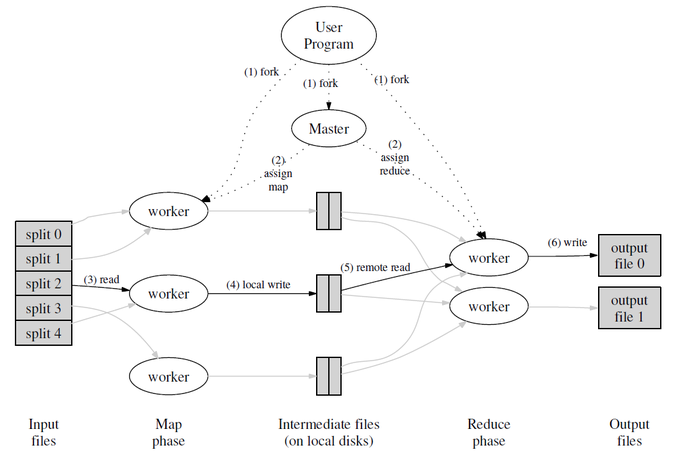
\includegraphics[scale=0.6]{images/mapreduce}
\caption{MapReduce schéma \cite{mapreduce}}
\label{fig:mapreduce}
\end{figure}

\newpage

\section{NoSQL}
Se zkratkou SQL se můžeme u relačních databázových systémů. Zkratka NoSQL neznamená pravý opak, písmena \uv{No} znamenají \uv{Not Only}, tedy ne pouze. Jedná se o databázový koncept, který se vyskytuje u nerelačních databází. V tomto konceptu datové úložiště i zpraování dat používají jiné prostředky, než běžné tabulkové schéma relační databáze. Výhody tohoto konceptu jsou jednoduchá desihn a horizontální i vertikální škálovatelnost. NoSQL databáze často podporují také podmnožinu jazyka SQL a většinou se jedná o jednoduché funkce jako vkládání a velice jednoduché výběry. Některé NoSQL databáze mají i velice odlišný ukládací model, například (stromový, grafový) tím padem je složitost  pro různé operace odlišná. Nejčastější podobu má NoSQL databáze formou klíč hodnota, čili mapa. Podle dosavadních informací lze říci, že Google BigTable je tedy NoSQL databáze. Mezi charakteristiky NoSQL databází můžeme zahrnout

\begin{itemize}
\item \textbf{Datový a dotazovací model} - jak již bylo řečeno NoSQL databáze se liší způsobem udržování dat a  dotazováním nad nimi
\item \textbf{Perzistence} - Ne všechny NoSQL datbáze ukládají svá data na disk, některé databáze běží pouze v operační paměti.
\item \textbf{Rozhraní} - Některé databáze komunikují skrze REST rozhraní a některé pomocí binárních protokolů 
\item \textbf{BASE} - Tak jako relační databáze využívají vlastnosti ACID (Atomic Consistent Isolation Durability) tak v NoSQL je ekvivalentem BASE (Basically Available, Soft state, Eventual consistency) kde každá NoSQL databáze garantuje jednotlivé vlastnosti různými mechanizmy a nastaveními nebo jsou již od základu navržené s danými vlastnostmi.   
\end{itemize}


NoSQL databáze jsou dalším základním stavebním kamenem BigData. NoSQL databáze jsou často kompatibilní s MapReduce konceptem, čímž tvoří ideální dvojici pro uchovávání a zpracování velkého množství dat. 



\chapter{BigData Platforma Apache}

V předchozí kapitole jsme se seznámili s technickými principy a postupy, které se uplatňujív BigData konceptu. V tét kapitole se budu zabývat jedním z hlavních témat práce a tou je open source řešení pro platformu BigData od organizace Apache Foundations, také známý jako Apache Big Data stack. Tento stack se skládá z několika aplikací, které až na jednu výjimku na sobě nejsou nikterak závislé. V záběru této kapitoly se budu důkladně věnovat pro nás nejdůležitější části tohoto stacku a tím je NoSQL databázový systém Cassandra.

\section{Hadoop}




Hadoop je softwarová knihovna napsaná v programovacím jazyce Java a umožňuje distribuované zpracování velkého množství dat napříč clusterem pomocí jednoduchých programovacíh modelů- Je navržený aby dobře škáloval cluster tvořící jeden až několik tisíc počítačů, kde každý nabízí lokální výpočetní výkon a úložiště dat. Hadoop řeší problémy s hardwarem na aplikační vrstvě a tudíž je možné navrhovat vysoce dostupné služby na clusterů počítačů, aniž bychom se museli strachovat výpadků. Jeho 4 komponenty tvoří nejpodstatnější část pro celou analytickou práci s  daty. A všechny ostatní aplikace přímo, čí nepřímo některé části Hadoopu používají nebo jsou na nich dokonce založeny. Jaké tedy jsou tyto 4 komponenty hadoopu ?


\begin{figure}[h]
\centering

\includegraphics[scale=0.15]{images/hadoop}
\caption{Logo Apache hadoop}
\label{fig:yarn}

\end{figure}


\subsection{Hadoop Commons}
Jedná se pouze o základní sadu nástrojů podporujícíc a propojující ostatní moduly Hadoopu.


\subsection{Hadoop File System (HDFS)}
Jedná se o open source distribuovaný filesystém, jehož některé prvky vychází z dříve zmíněného GFS. HDFS umožňuje uložit velké množství dat mezi jednotlivé uzly.  HDFS umožňuje velice dobré škálování s rostoucím objemem dat. Ostatní technologie z Apache Big Data Stacku filesystém využívají ke sběru a ukládání výsledků jejich analytických procesů. HDFS cluster se skládá primárně z NameNode, který řídí filesystemová metadata a z DataNodů, které data uchovávají. 

\subsection{Hadoop MapReduce}
MapReduce jsme zmínili výše a jen zopakuji, že se jedná o programovací paradigma a framework na paralelní zpracování dat. Nabízí API, díky kterému můžeme jednoduše programovat naše vlastní MapReduce operace. Tento framework nabízí základní kostru, kterou programátor doplní a o vše ostatní se stará samotná knihovna. Přesto všakveškerá logika programu zavisí na programátorovi. 

\subsection{Hadoop YARN}
Tento modul se stará o plánování jednotlivých MapReduce programů a o správu dostupných zdrojů v celém clusteru a rozhoduje jaká data se kam budou posílat a počítat. Základní Architektura YARNu má za myšlenku mít jeden globální uzel, který se nazývá \uv{Resource Manager} a Pro každý běh aplikace mít tzv. \uv{Application Master}, který má na starosti komunikaci s \uv{Node Managery} a dohlížením nad spouštěním jednotlivých Tasků. Resource Manager se skládá ze 2 hlavních komponent Plánovače a Aplikačního manažera. Plánovač je zodpovědný za alokování zdrojů pro různé běžící aplikace. Aplikační manažer je zodpovědný za příjem nových MapReduce programů a jejich správné zařazení. NodeManager je agent běžící na každém stroji, která je zodpovědný za aplikační kontejnery a monitoruje stav dostupných prostředků stroje a ohlašuje se Resource Manageru, který tak má potřebné informace k přerozdělování nových úkolů.

\begin{figure}[h]
\centering
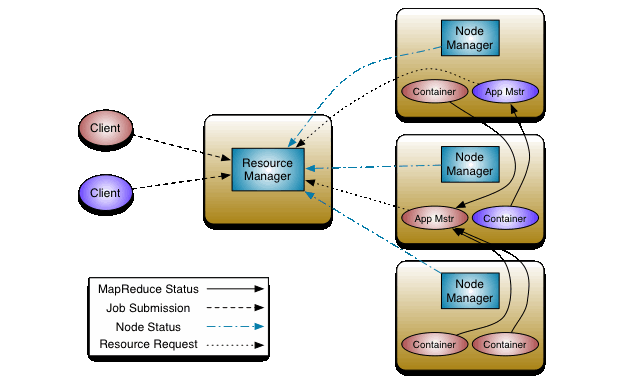
\includegraphics[scale=0.7]{images/yarn_architecture}
\caption{Architektura Hadoop YARN}
\label{fig:yarn}

\end{figure}



\newpage 

\section{HBase}
Je NoSQL databázový systém, který je založený na principu Google BigTable. Jedná se o druhou nejpoužívanšjí NoSQL databázi v Apache Big Data Stacku. Implementačně je zavíslá na HDFS, který používá k ukládání dat. Výhodou je velice jednoduhá a rychlá integrace s Hadoop MapReduce. HBase sdědil po Hadoopu i jeho Master-Slave architekturu.


\section{Hive}


Apache Hive je data warehouse infrastruktura postavená na vrchu Hadoopu na poskytování analýzy a dotazování se nad daty. Původně byl tento software vyvinut ve společnosti Facebook. A nyní se jeho starají společnost jako je NetFlix a Amazon. Hive podporuje anaýzu velkých datasetů uložených v HDFS nebo HDFS-kompatibilních systémech jako například (CassandraFS nebo Amazon S3). Syntaxe jeho dotazovacího jazyka HiveQL je velice podobná SQL a proto ho mohou inženýři ovládající tento jazyk velice brzy ovládnout.HiveQL nabízí programátorům prostředky, které nejsou běžně v NoSQL databázích dostupné jako například funkce JOIN. 

\begin{wrapfigure}{r}{0.5\textwidth}
  \centering
    
\includegraphics[scale=0.5]{images/hive_logo}
\caption{Logo Apache Hive}

\end{wrapfigure}

Hive funguje na principu, že si dotaz přeloží a převede do kodu kompatibilního s Hadoop Mapreduce a výsledný program následně spustí na Hadoop clusteru. Obrovskou výhodou je, že programátor dostává v podstatě s nulovým snažením hotový MapReduce program, který by jinak musel zdlouhavě psát, což umožnuje být vysoce efektivní. Hive si standardně ukládá metadata do embedované databáze Derby. Podporuje pokročilejší funkce jako například Indexy, kompresi nebo uživatelem definované funkce (UDF) samozřejmostí jsou standardní matematické a řetězcové funkce aplikovatelné v HiveQL dotazech. 



\section{Pig}


Pig funguje na stejném principu jako Hive. Tedy , že převede vámi napsaný kód do hotového MapReduce řešení a tento kód spustí nad Hadoop clusterem. Tato knihovna byla napsána ve firme Yahoo a později opensourcována pod Apache foundation. Pig používá svůj vlastní jazyk pojmenovaný Pig Latin a oproti HiveQL nemá s SQL moc společných rysů. Latin se spíše podobá funkcionálním jazykům. Pig a Hive dělají tedy stejné věci, tak proč používat obojí? Je to spíše volba osobních preferencí, či preferencí vašeho vývojářského týmu. S oběma technologiemi lze dosáhnout stejných výsledků. Přesto má Pig lepší uplatnění v případě tvorby komplikověnšjích data flow a HiveQL se více hodí pokud jsou potřeba Ad-Hoc dotazy. Přestože lze dosáhnout stejných výsledků s oběmi platformami, určitě doporučuji umět obě a použít Hive nebo Pig v konkrétních siuacích, kde mají lepší užití. 



\section{SolR}

Solr [Solar] je vyhledávací platformou odvozenou od Apache Lucene. Mezi její hlavní výhody patří:

\begin{itemize}
\item Pokročilý full-text vyhledávací engine
\item Optimalizace pro vysokoobjemový tok dat
\item Otevřené rozhraní pomocí XML,JSON nebo HTTP
\item Lineární škálovatelnost, automatická replikace indexu, auto failover a samoobnovení
\item Indexace v témeř reálném čase
\item Možnost doprogramování vlastních pluginů
\end{itemize}

Solr využívá Lucene index, což znamená, že je formát je striktně definovaný. Změna ve formátu indexu znamená reindexaci celého dokumentu. Díky lehkému nastavení a možnostem výstupu a pokročilými funkcemi jako je například GeoSpatial vyhledávání nebo facetové full text hledání, je SolR v komerční a open source sféře vyhledávacím enginem číslo 1.


\section{Squoop}

Tento nástroj je velice užitečný, protože ne vždy chceme mít všechna data pouze v NoSQL databázích a pokud to je možné, využití výhod relačních databází je logickou volbou. Apache Squoop je nástroj pro hromadnou migraci z HDFS (či kompatibilního) file systému do strukturovaných úložišt jako například: relačních databází. Přesun dat je navržený obousměrně stejně tak můžeme využít Squoop k migraci dat z  relačních databází do HDFS (a kompatibilních) systémů. Výhodou je vysoká efektivita a nízká časová investice oproti psaní vlastních migračních scriptů.

\section{Mahout}

Mahout je slovo, které pochazí z Hindi a jeho překladem do češtiný získáme spojení jezdec na slonovi. Slonem se v BigData komunitě myslí projekt Apache Hadoop, který má slona ve svém logu a je s tímto zvířetem neodmyslitelně spojený. Projekt Mahout se snaží svým metaforickým názvem naznačit využívání hadoopu k vytvoření knihovny pro podporu škálovatelného \uv{Machine learningu}. Mahout je sada funkcí a algoritmů využívaných v odvětví machine learningu, naprogramovaných pomocí Hadoop MapReduce paradigmatu. Primární zaměření Mahoutu je na odvětví kolaborativního filterování, clusterování a klasifikace dat. Mahout také obsahuje vysoké množství matematických funkcí a algoritmů z oblasti lineární  algebry a statistiky. V současné době lze využít Mahout na tyto základní způsoby užití. Doporučovací funkce na základě uživatelského chování, rozřazování dokumentů do clusterů na základě shody v obsahu a Klasifikace dokumentů na základě již uložených kategorizovaných dokumentů. 

\section {ZooKeeper}

Autoři projektů v rámci Apache foundations a především ti zaměření na projekty BigData stacku mají pro metafory a různá symbolická spojení velkou slabost. Jak názvy a loga projektů napovídají, velká část projektů má v názvu nebo logu nějaké zvíře, či referenci na něj. Zároveň uhlídat a spravovat byť malý ale distribuovaný systém, může být velký chaos a proto je potřeba ten správný hlídač. ZooKeeper v překladu tedy hlídač zoo je nástroj pro správu a konfiguraci distribuovaných systému z platformy Apache BigData. 



\chapter{Cassandra}	


V předchozí kapitole jsme rozebrali veškerý software z Apache Big Data Stacku kromě jednoho. Cassandra je NoSQL WideColumn databáze a jedná se o nejdůležitější software z Apache Big Data Stacku z pohledu této práce, která se právě na Cassandru zaměřuje. Z tohoto důvodu tuto databázi nyní do detailu rozebereme. 

\section{Proč Cassandra}
Přestože NoSQL databází vhodných k uchovávání a zpracovávání BigData existuje celá řada, vybral jsem si Cassandru, protože si myslím, že je nejzajímavější z hlediska architektury. Dosahuje skvělých výsledků v porovnávacích testech\cite{benchmark}, používají ji v produkci a velikých clusterech známé společnosti, má největší komunitu (a na vývoji se aktivně podílejí i velké firmy) a je nejpoužívanější databází ve své kategorii\cite{dbengines}. V neposlední řadě také proto, že jsem se s touto databází setkal již dříve a chtěl jsem zjistit, kam se databáze za tu dobu pohnula.

Díky široké nabídce funkcí a výše popsaným důvodům si myslím, že je tato databáze vhodná i pro edukační účely zejména pro její jednoduchost a zároveň komplexnost. Vzhledem k jednoduchosti začlenění s ostatním softwarem z Apache Big Data Stacku se stává z Cassandry ultimátní BigData nástroj. Absolventům může přijít vhod také fakt, že Cassandra je průmyslově nejpoužívanější databází svého druhu. %citace?


\section{Vznik}

Cassandra vznikla v roce 2008 ve společnosti Facebook, kde sloužila jako úložiště zpráv mezi uživateli této obří sociální sítě. Facebook později téhož roku uvolnil zdrojové kódy projektu. Projekt se v roce 2009 dostal do inkubační fáze pod záštitou Apache Foundation. O rok později – v roce 2010 – se projekt dostal mezi plnohodnotné projekty Apache Foundation. Jak již bylo zmíněno, velké rozdíly mezi verzemi jednotlivých projektů z Apache Big Data Stacku způsobují závažné problémy s kompatibilitou celého systému. Ani Cassandra není výjimkou, i její rozdílné verze nesou rizika a rozdílné funkce a samozřejmě také nekompatibilitu. V současné době je nejaktuálnější verzí Cassandra 2.04 a pokud nebude uvedeno jinak, uvažujeme v textu tuto verzi. 

\section{Předchůdci}

Když Facebook vydal článek popisující Cassandru \cite{facebookcassandra}, popsal ji jako \uv{To nejlepší z Google BigTable a Amazon DynamoDB}, což není náhoda, neboť prvotním šéfem vývoje Cassandry ve Facebooku byl právě inženýr, který ve společnosti Amazon navrhl a vytvořil databázi Dynamo. Podoba s BigTable také není náhodná, Facebook pro své potřeby potřeboval wide-column databázi, a proto byla inspirace BigTable přirozenou volbou. 

\subsection{Co Cassandra zdědila od Dynama}
\begin{itemize}
\item \textbf{Symetrie} Každý uzel má stejnou zodpovědnost a roli v systému.
\item \textbf{Decentralizace} Rozšíření symetrie. Každý uzel může plně komunikovat s jakýmkoliv jiným uzlem a získávat od něj informace. Je tedy možné ovládat systém skrze kterýkoliv uzel, což přispívá k výborným škálovacím vlastnostem. 
\item \textbf{Heterogenita} Každý uzel může mít jiné vlastnosti (např. kapacitu disků) a přidání nového uzlu s jinými vlastnostmi by tím pádem nemělo systém nikterak ohrozit. 
\end{itemize} 

\subsection{Co Cassandra zdědila od BigTable}
\begin{itemize}
\item \textbf{Datový model} Stejně jako BigTable má Cassandra Wide-Column schéma reprezentované klíčem a hodnotou.
\item \textbf{Distribuovaný log} K zápisu používá databáze interně distribuovaný \uv{append log}. 
\end{itemize} 

\section{Kdo Cassandru používá v produkci}

Cassandru v produkčním nasazení můžeme nalézt u mnoha významných společností, které ji používají v clusterech s velikostí od pár uzlů až po největší známý Cassandra cluster o velikosti 400 uzlů a 300 TB dat. Mezi nejznámější společnosti patří:

\begin{itemize}
\item Twitter
\item Ebay
\item Spotify
\item NetFlix
\item Cisco
\item Urban Airship
\item Reddit
\item Accenture
\item a mnoho dalších…
\end{itemize} 

\begin{figure}[h]
\centering

\includegraphics[scale=0.45]{images/casa-production}
\caption{Ukázka ostatních firem využívajících Cassandru v produkčním prostředí}
\label{fig:yarn}
\end{figure}


\section{Společnosti vyvíjející Cassandru}
Cassandra je open source projekt, který je ovšem rozvíjen dvěma velkými společnostmi Acunu a Datastax. Především druhá jmenovaná společnost má na vývoji a budoucnosti Cassandry velkou zásluhu. Datastax pořádá školení a certifikuje vývojáře a administrátory, pořádá setkání a především Cassandru přidává do svého komerčního BigData balíčku, který je nadstavbou Apache Big Data Stacku přidávající vlastní funkcionalitu a spojující všechny komponenty v jeden funkční celek. Pro nekomerční užití v testovacích prostředích je tento balíček k dispozici zdarma.
\section{Hlavní výhody}

Cassandra nabízí pro vývojáře mnoho lákadel. Nyní tu vypíši ty nejzajímavější, které si později rozebereme ve větším detailu. 

\begin{itemize}
\item \textbf{Replikace} Systém sám replikuje data podle kriterií, která mu zadáme.
\item \textbf{Transparentní škálování} Programátor může napsat kód proti lokální instanci a aplikace bude fungovat v jakémkoliv clusteru.
\item \textbf{Nastavitelná konzistence} Můžeme měnit nastavení konzistence přímo za běhu aplikace.
\item \textbf{Nastavitelná síťová strategie} Správce může definovat strategii, podle které systém pozná, do jakého datacentra (případně racku) má uzel zařadit.
\item \textbf{Cassandra Query Language (CQL)} Dotazovací jazyk velmi podobný SQL
\item \textbf{MapReduce} Podpora Hadoop MapReduce
\item \textbf{Databáze nemá \uv{Single Point of Failure}} Díky plně P2P architektuře není databáze náchylná na výpadek jakéhokoliv uzlu.
\item \textbf{Rychlost} Čtení i zápis dosahuje skvělých výsledků \cite{benchmark} a to i při lineárním škálování. 
\end{itemize} 

\begin{figure}[h]
\centering
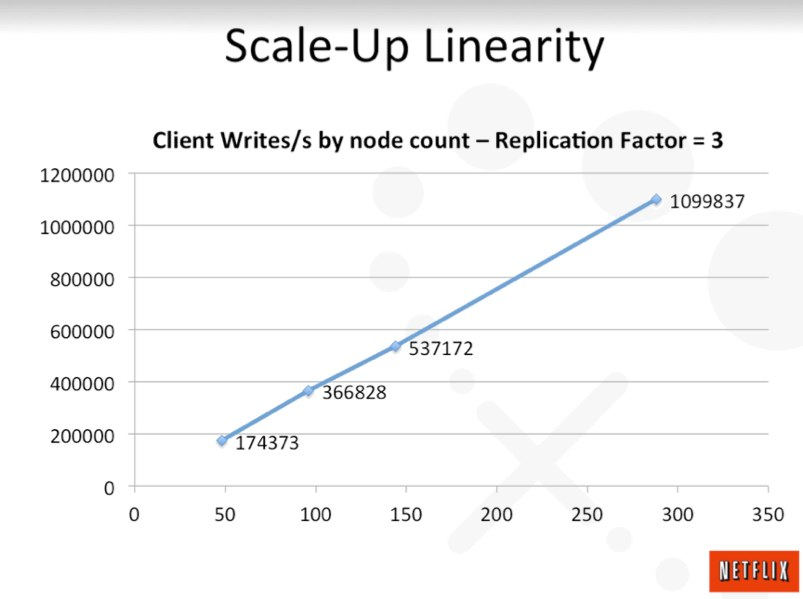
\includegraphics[scale=0.5]{images/netflix}
\caption{Škálování Cassandry a vliv na I/O operace}
\label{fig:scaleup}
\end{figure}

\section{Architektura}
Architektura Cassandry se skládá z několika klíčových bodů, z nichž každý plní svou roli. V následujících podsekcích je stručně vysvětlím.

Cassandra je plně symetrický systém, kde neexistuje jediný bod selhání. Její architektura byla navržena s premisou, že podpůrný hardware a software může padat. Právě proto Casandra nabízí symetrickou architekturu, kde jsou si všechny uzly rovny a veškerá data jsou uložena napříč všemi uzly v clusteru. Commit logy na každém uzlu zachycují veškeré zápisy a data jsou rovněž ukládána do mezipaměti. Když dojde k jejímu zaplnění, tak se data zapíší na disk a automaticky zreplikují a následně rozdistribuují po celém clusteru. 

Klientské požadavky na zápis nebo čtení mohou přijít na kterýkoliv uzel z clusteru a ten se pak pro daný požadavek stává koordinátorem, který se stává jakousi proxy mezi klientem a uzlem, který data vlastní. Tato architektura nám zajišťuje lineární škálování viz \ref{scaleup}

\subsection{P2P protokol \uv{Gossip}}
Do češtiny bychom mohli název tohoto protokolu přeložit jako štěbetání nebo klábosení. Tento název je vlastně velmi trefný, neboť to je v podstatě právě to, co spolu servery dělají. Plně Peer to peer architektura systému s protokolem, kde si jednotlivé uzly o sobě sdělují všechny informace nám dává k dispozici systém, kde každý uzel ví, kde má hledat která data, který uzel je nedostupný, a kterému uzlu by měl nějaká data poslat. Když do systému připojíme nový uzel, ostatní uzly ho ihned začnou zahrnovat informacemi o všech ostatních uzlech v clusteru. To samé platí i pro uzly, které se do clusteru vrátí po nějakém výpadku. Každý uzel o sobě ostatním uzlům posílá informace každou vteřinu. Každý uzel pošle informaci o sobě a ostatních až 3 uzlům najednou a informace sebou nese i časové razítko, aby se předešlé informace mohly přepsat. Tímto způsobem se všechny clustery velice rychle dozví veškeré informace o všech ostatních uzlech v clusteru. 

Pokud je uzel označený jako nefunkční, Cassandra na něj neposílá žádně požadavky. Stejně tak může neposílat požadavky na funkční, ale příliš vytížený uzel pomocí dynamického prohledávání. Zapisování dat, o která uzel přišel po dobu svého výpadku, rozebereme v jedné z dalších sekcí. 

\subsection{Rozdělovač}
Rozdělovače (anglicky \uv{partitioner}) určují, jakým způsobem budou data a jejích repliky rozloženy po clusteru. Jednoduše řečeno, jedná se o hashovací funkci, která vezme klíč, jež chceme ukládat a vrátí nám token, podle kterého určíme, na jaké uzly se má tato hodnota zapsat. Na výběr máme ze 3 možností:

\begin{itemize}
\item \textbf{Murmur3Partitioner} - jedná se o počáteční hodnotu, která rozmisťuje data rovnoměrně po clusteru na základě MurMur3 hashovací funkce.
\item \textbf{RandomPartitioner} - rovnoměrně umisťuje data po clusteru na základě MD5 hashovací funkce (je pomalejší než MurMur3).
\item \textbf{ByteOrderedPartitioner} -  Ukládá data po clusteru na základě lexikálního pořadí bytů. Nedoporučuje se kvůli složitému vyvažování a nerovnoměrné distribuci dat. Jedinou výhodou je sekvenční hledání podobných klíčů.
\end{itemize}

\subsection{Distribuce a replikace dat}
Když si zvolíme vhodný rozdělovač, na základě kterého určujeme, kam příslušný klíč patří, musíme serverům přiřadit určitou výseč klíčů. 

\subsubsection{Kruh}
V Cassandře uzly tvoří takzvaný kruh. Podle počtu uzlů v kruhu se vypočte výseč tokenů, které danému uzlu patří. 

\subsubsection{Virtuální uzly}
Cassandra od verze 1.2 přináší zásadní vylepšení v podobě virtuálních uzlů, kde se každý uzel rozdělí na několik virtuálních (každý dostane svou náhodnou výseč), čímž se rapidně snižuje počet tokenů, které uzlu patří. Virtuální uzly zlehčují a vylepšují v Cassandře hned několik úkonů:

\begin{itemize}
\item Tokeny pro nové uzly se přiřazují náhodně samy a pro nové uzly již tedy není nutné tokeny počítat a přiřazovat manuálně.
\item Oprava mrtvého uzlu je mnohem rychlejší, jelikož se na ní podílí všechny ostatní uzly v clusteru a změny probíhají inkrementálně.
\item Po přidání nového uzlu nemusíme dělat složité převažování clusteru, virtuální uzly se vytvoří rovnoměrně mezi ostatními uzly a vezmou si tak od každého uzlu mnohem menší objem dat.
\item Zlepšuje využití heterogenních strojů v clusteru. Strojům s rozdílnou kapacitou můžeme nastavit rozdílný počet virtuálních uzlů.
\end{itemize}

\begin{figure}[h]
\centering
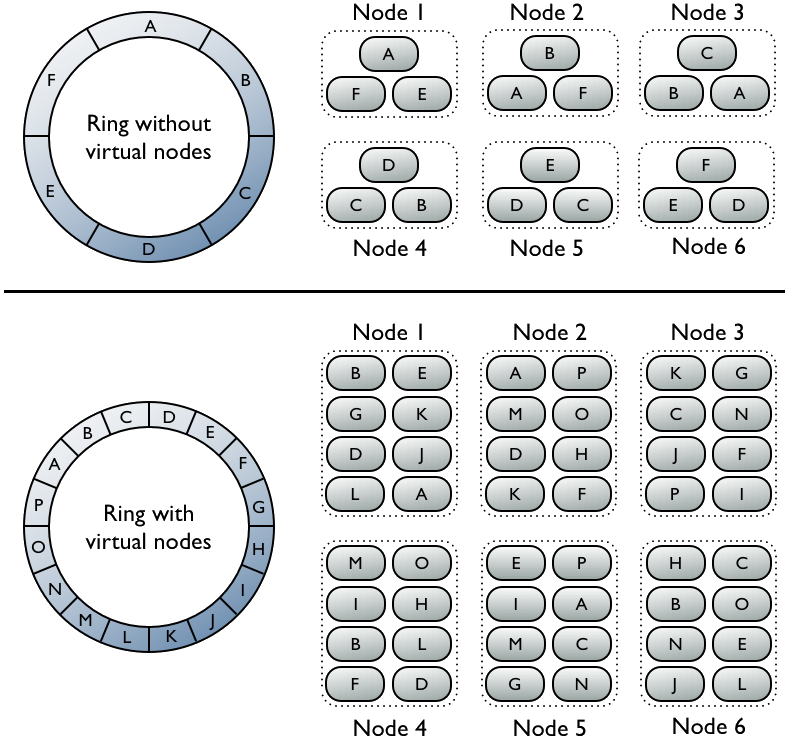
\includegraphics[scale=0.5]{images/vnodes_compare}
\caption{Porovnání uložení dat v kruhu s a bez virtuálních uzlů}
\label{fig:vnodes}
\end{figure}

Když má každý (virtuální) uzel přiřazenu svou množinu tokenů a máme určeno, jak budeme tokeny získávat, je potřeba vyřešit replikování dat. Počet replik je daný replikačním faktorem, který se nastavuje pro každou databázi. Replikační faktor 1 znamená, že každá řádka bude existovat pouze jednou. Replikační faktor 2 znamená, že každá řádka bude uložena dvakrát a pokaždé na jiném stroji. V Cassandře jsou si všechny uzly rovny a to stejné platí také pro repliky dat. Neexistuje tedy žádná hlavní replika, všechny jsou stejně důležité. Replikační faktor by neměl překročit maximální množství uzlů v clusteru, data by pak byla redundantní a ztráceli bysmevýkon. Na výběr máme ze dvou replikačních strategií:


\begin{itemize}
\item \textbf{Jednoduchá strategie} - Využívá se pouze pro clustery uložené v jednom datovém centru. Tato strategie uloží první repliku na uzel určený rozdělovačem a ostatní repliky jsou uloženy na následujících uzlech v kruhu po směru hodinových ručiček bez ohledu na topologii (pozice v racku či datacentru).
\item \textbf{Síťová strategie} - Globální replikační faktor se zde změní na replikační faktor pro každé datacentrum. Každé datacentrum má vlastní kruh. Rozmisťování kopií tedy funguje následovně: První kopie se uloží na uzel vybraný rozdělovačem a další kopie ve stejném datacentru se uloží na nejbližší uzel po směru hodinových ručiček, který se nachází v jiném racku. 
\end{itemize}

\subsection{Donašeči (Snitches)}
Donašeči informují Cassandru o síťové topologii clusteru. Smyslem je, aby požadavky byly směřovány efektivně a aby repliky mohly být uloženy do různých racků či datacenter. 

Na výběr máme několik implementací od jednoduchých, řešících topologii sítě maskováním IP adresy, až po komplexní, kde definujeme topologii ručně. Cassandra nabízí implementace i pro známé cloudové řešení od Amazonu, které dokáže rozeznávat i jednotlivé regiony tohoto poskytovatele.

\subsubsection{Dynamické donášení}
Všechny implementace mají implicitně zapnutou tuto volbu, která se snaží omezit čtení z aktuálně přetížených uzlů směrováním požadavků jinam a chytře tak využívá celý cluster. 

\subsection{Úrovně konzistence}
Cassandra nabízí různé úrovně konzistence pro čtení i zápis. Možné hodnoty a jejich vlastnosti jsou popsané v tabulce \ref{casareads} a tabulce: \ref{casawrites}

\begin{table}
  %  \begin{tabular}{|l|l|}
\begin{tabularx}{\textwidth}{ |l|X| }

    \hline
    Úroveň       & Popis                                                                                                                                                                                                                                                                                  \\ \hline
    ANY          & Zápis se musí provést alespoň na jeden uzel. Pokud jsou všechny uzly, kam má být replika umístěna, nedostupné, můžeme provést zápis do odkladového úložiště. Tyto data však nebudou přístupná ke čtení do té doby, než alespoň jeden uzel vlastnící repliku těchto dat nebude dostupný. \\ \hline
    ONE          & Data musí být zapsána do commit logu a paměti alespoň jednoho uzlu, kde má být replika umístěna                                                                                                                                                                                        \\ \hline
    TWO          & Data musí být zapsána do commit logu a paměti alespoň dvou uzlů, kde má být replika umístěna                                                                                                                                                                                           \\ \hline
    THREE        & Data musí být zapsána do commit logu a paměti alespoň tří uzlů, kde má být replika umístěna                                                                                                                                                                                            \\ \hline
    QUORUM       & Data musí být zapsána do commit logu a paměti na větší polovině uzlů, kde má být replika umístěna                                                                                                                                                                                      \\ \hline
    LOCAL\_QUORUM & Data musí být zapsána do commit logu a paměti na větší polovině uzlů, kde má být replika umístěna v datacentru koordinátorského uzlu.                                                                                                                                                   \\ \hline
    EACH\_QUORUM & Data musí být zapsána do commit logu a paměti na větší polovině uzlů, kde má být replika umístěna v každém datacentru.                                                                                                                                                                  \\ \hline
    ALL          & Data musí být zapsána do commit logu a paměti na všech uzlech, kde má být replika umístěna.                                                                                                                                                                                             \\ \hline
    \end{tabularx}
    \caption {Úrovně konzistence pro zápis}
\label{casawrites}

\end{table}


\begin{table}[!h]
%    \begin{tabular}{|l|l|}
\begin{tabularx}{\textwidth}{ |l|X| }

    \hline
    Úroveň       & Popis                                                                                                                    \\ \hline
    ONE          & Vrátí odpověď z nejbližšího uzlu a na pozadí spustí opravné čtení                                                        \\ \hline
    TWO          & Vrátí aktuální data z dvou nejbližších uzlů (majících repliky)                                                           \\ \hline
    THREE        & Vrátí aktuální data ze tří nejbližších uzlů (majících repliky)                                                           \\ \hline
    QUORUM       & Vrátí nejnovější data poté, co odpoví větší polovina uzlů majících repliky                                               \\ \hline
    LOCAL\_QUORUM & Vrátí nejnovější data poté, co odpoví větší polovina uzlů majících repliky ze stejného datacentra v jakém se nachází koordinátor \\ \hline
    EACH\_QUORUM & Vrátí nejnovější data poté, co odpoví větší polovina uzlů majících repliky z každého datacentra                          \\ \hline
    ALL          & Vrátí nejnovější data poté, co odpoví větší polovina všech uzlů majících repliky                                         \\ \hline
    \end{tabularx}
    \caption {Úrovně konzistence pro čtení}
\label{casareads}

\end{table}


\subsection{Eventuální konzistence}
Cassandra disponuje eventuální konzistencí, což znamená, že úroveň konzistence je proměnlivá. Cassandra tímto obchází zažité paradigma CAP teorému a implementuje tak segmentovanou konzistenci, kterou jsme popisovali dříve. Je na architektovi (a případně vývojáři), kdy jakou úroveň konzistence použije. Cassandra umožňuje zvolit konzistenci pro každý požadavek zvlášť, dokonce i pokaždé jinou pro stejný dotaz. Toto dává architektům a vývojářům obrovskou výhodu při návrhu i samotné implementaci. 

\subsection{Výběr vhodné konzistence}
Univerzální pravidlo pro výběr vhodné úrovně neexistuje, záleží vždy na konkrétní situaci a akci. Obecně ovšem platí, že pokud potřebujeme data rychle, volíme nižší úrovně, naopak pokud vyžadujeme co nejaktuálnější data, použijeme nejvyšší úrovně. 

\section{Klientské dotazy}
Jak bylo zmíněno v předchozích sekcích, Cassandra je plně symetrický systém a tudíž požadavky (jak na čtení, tak zápis) mohou přicházet na kterýkoliv (!) uzel v clusteru. Uzel, který požadavek přijme, se stává koordinátorem a zajišťuje, aby byl úspěšně dokončen. Koordinátor určuje, který uzel vlastní která data na základě rozdělovací a replikační strategie. 

\subsection{Zápis}
Koordinátor pošle požadavek o zápis na \textbf{všechny} uzly, které podle rozdělovací a replikační strategie vlastni tato data. Na tyto uzly budou data zapsána nehledě na úroveň konzistence. Konzistence nám určuje, na kolik odpovědí od uzlů bude koordinátor čekat, než ohlásí požadavek za úspěšný. Úspěšný zápis znamená, že data byla zapsána do commit logu a do mezipaměti. 

Představme si modelovou situaci, kdy máme cluster o 12 uzlech a data zapisujeme s úrovní ONE a replikační faktor máme 3. Koordinátor (v tomto případě uzel 10) pošle požadavek o zápis na uzly 1, 2 a 7. Koordinátor prohlásí požadavek za úspěšný, když mu přijde první odpověď od kteréhokoliv uzlu.

\begin{figure}[h]
\centering
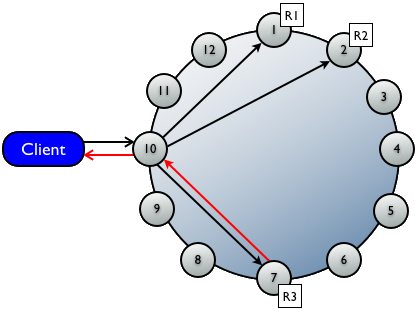
\includegraphics[scale=0.5]{images/write}
\caption{Ukázka zápisu dat s replikačním faktorem 3 a konzistencí 1}
\label{fig:vnodes}
\end{figure}


\subsection{Čtení}
Čtení probíhá dvěma možnými způsoby:

\begin{itemize}
\item Přímé čtení probíhá podobně jako zápis a podrobněji ho rozepíšeme níže.
\item Čtení a opravení dat na pozadí. Jedná se o složitější mechanismus, který popíšeme v následující sekci.
\end{itemize}

Jak již bylo řečeno, přímé čtení funguje podobně jako zápis. Koordinátor odešle požadavek na získání dat všem uzlům, které data vlastní a úroveň konzistence určuje, na kolik správných odpovědí budeme čekat. Data v uzlech mohou být nekonzistentní, Cassandra považuje za správná ta nejnovější data. Konzistenční úroveň u čtení tedy říká, kolik uzlů mi musí vrátit aktuální data. 

V následujícím příkladu uvažujeme stejný cluster jako při zápisu a vyžadujeme data s konzistenční úrovní QUORUM. 2 ze 3 uzlů nám vrátily aktuální data a tedy považujeme celý požadavek za úspěšný. Koordinátor vrátí klientovi data.


\begin{figure}[h]
\centering
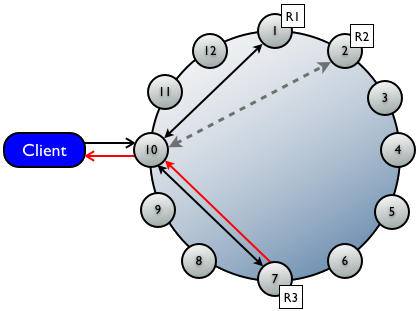
\includegraphics[scale=0.55]{images/read}
\caption{Ukázka čtení dat s replikačním faktorem 3 a konzistencí Quorum}
\label{fig:vnodes}
\end{figure}


\section{Zachování konzistence}%end
Jak bylo naznačeno, při zápisu se může stát, že je uzel nedostupný a nedostane tedy data, která by měl zapsat a tím vznikají nekonzistence dat. Cassandra má 3 interní mechanismy jak si s nekonzistencí dat poradit: 

\begin{itemize}
\item \textbf{Read Repair} Pokud Cassandra při čtení zjistí, že má nějaký uzel nekonzistentní data, pošle po dokončení požadavku na pozadí aktualizační požadavek a data na těchto uzlech aktualizuje. Tato možnost je konfigurovatelná.
\item \textbf{Anti Entropy Node Repair} Pokud byl uzel dlouho nedostupný, můžeme spustit opravný nástroj, který se sám dotáže na konzistenci dat ostatních uzlů a postupně je opraví. 
\item \textbf{Hinted Handoff} Pokud se stane, že je některý z uzlů nedostupný během zápisu, ostatní uzly s replikami si uloží takzvaný hint ohledně zápisu a ve chvíli, kdy se pomocí Gossip protokolu dozví, že daný uzel se vrátil zpět do clusteru, pošlou mu informaci o zápisu. Pokud použijeme při zápisu úroveň konzistence ANY, můžeme zápis provézt úspěšně i pokud budou všechny uzly, kterým data patří, nedostupné. Data a hint se v takovém případě uloží na koordinátorském uzlu. Tato data ovšem nebudou dostupná ke čtení, dokud nebudou řádně zapsána alespoň do jednoho z uzlů kam patří.
\end{itemize}

\section{Oprava dat na disku}
Přestože detailní struktura a ukládání dat na disku je nad rámec tohoto textu, je vhodné říci, že díky své struktuře zděděné od BigTable neprovádí Cassandra žádné inplace úpravy ani mazání. Místo toho používá náhrobky a nové zápisy s aktuálnějšími daty a časovým razítkem. Z toho plyne, že z hlediska zlepšení výkonu a ušetření místa na disku je potřeba čas od času provést pročištění a sjednocení těchto \uv{append-only} souborů. Této technice se říká kompakce a jedná se o pokročilejší administrátorskou úlohu při práci s Cassandrou, která se nachází mimo rámec tohoto textu. %inplace?

\section{Datový model}
Reprezentaci dat a ukládací engine si Cassandra vypůjčila a přizpůsobila od BigTable. Cassandra tedy spadá pod Key-Value storage systémy a WideColumn systémy. Těmto systémům se občas nadlehčeně říka\uv{Fancy hash table}, což můžeme přeložit jako \uv{Honosná HashTabulka}. Důvodem pro toto lehce posměšné označení je jednoduchý princip celého datového modelu, tedy že se jedná \uv{pouze} o ukládání klíče-hodnoty s pár funkcemi navíc. Vzhledem k vyspělosti těchto systémů v dnešní době a rozsáhlosti funkcí, můžeme toto dehonestující označení považovat za pouhý komunitní slovní žert.

Cassandra v dnešní době disponuje moderním rozhraním, které si popíšeme v další sekci. Považuji však za vhodné si připomenout takzvané \uv{legacy API}, které plně odkrývalo reprezentaci dat, jež je důležitá pro pochopení toho, jak vlastně Cassandra funguje uvnitř. V dnešní době je tento engine obalen příjemným SQL-Like rozhraním. Znalosti \uv{legacy API} se nám však mohou hodit při návrhu našeho doménového modelu a optimalizaci dotazů. V neposlední řadě ještě i dnes můžeme použít toto staré Thrift API pro komunikaci s databází. Jak si ale brzy ukážeme, není k tomu žádný rozumný důvod. 

\subsection{Změna myšlení}
Pro uživatele přicházející ze světa relačních databází byl velký problém se vypořádat s úplně jiným přístupem a neubránili se neustálému srovnávání přístupů a pojmů. Pro ovládnutí principů NoSQL (a především efektivního a funkčního návrhu modelů v Cassandře) je důležité myslet na 2 hlavní zásady: 

\begin{itemize}
\item \textbf{Denormalizace} Vše, co jste se učili v SQL systémech o normalizaci dat, zde neplatí. Naopak by takové postupy vedly k nefunkčnímu návrhu. Cassandra neumí JOIN příkazy, které při normalizaci obvykle potřebujete a především NoSQL návrh vyžaduje vzhledem ke své nátuře úplně jiný přístup. 
\item \textbf{Redundance} Tento bod částečně souvisí s normalizací, která nám redundanci dat zakazuje a snaží se jí předejít. Při návrhu NoSQL systémů se držíme paradigmatu, které říká, že redundance dat nevadí, protože cena za mírné navýšení místa na disku je mnohem nižší, než cena za čas a HW potřebný ke spuštění takových dotazů, které by zvládly získat potřebná data bez redundance. Ukládat tedy některá data dvakrát za účelem jejich následného snadného čtení je doporučený postup. 
\end{itemize}

Tento přístup byl pro mnoho vývojářů tězce akceptovatelný a stal se jedním z důvodů, proč Cassandra používá CQL, o kterém si povíme později. I přes všechny její nadstavby je stále užitečné vědět, jak Cassandra funguje interně a navrhovat tak kvalitní datové modely. 

\subsection{základní stavební kameny}
Přestože jsme se chtěli od relačního databázového světa oprostit, pro vysvětlení některých pojmů je nejjednodušší srovnání, a proto v několika následujících bodech přirovnání k relačním databázím využiji.

\begin{itemize}
\item \textbf{Keyspace} - Udržuje pohromadě všechny Column Family a replikační faktor, který se na CF přenáší. Každý Keyspace může mít jiný replikační faktor. Keyspace se dá chápat jako pojem \uv{databáze} z relačního světa. Také má nějaké vlastnosti a ty platí pro všechny Column Families (tabulky), které sdružuje.
\item \textbf{Column Family} - Column Family sdružuje řádky, které obsahují sloupce. V relačním světě bychom mohli CF přirovnat k tabulce, která sdružuje jednotlivé záznamy. 
\item \textbf{Row} - Row je řádka identifikována jednoznačným klíčem (primárním) a obsahuje jednotlivé sloupce s daty. Každá řádka může obsahovat sloupce s odlišnými daty, řádky tedy nemají pevnou strukturu. Řádky bychom mohli přirovnat k jednotlivým záznamům v tabulce relační databáze, ale s tím rozdílem, že řádky v Cassandře nemají pevný formát. 
\item \textbf{Column} - Sloupec je nejmenší a tím pádem finální entitou udržující data v Cassandře. Sloupec má svůj název a hodnotu. Sloupce mají také časové razítko, které určuje čas vložení a dle něj se koordinátoři rozhodují, zda jsou sloupce z různých uzlů aktuální či nikoliv. Cassandra disponuje těmito druhy sloupců:

\begin{itemize}
\item \textbf{Standard} - Standardní obyčejný sloupec, který uchovává jednu hodnotu.
\item \textbf{Composite} - Spojený sloupec se používá, pokud je primární klíč složený z více sloupců. Názvy sloupců v takovém případě obsahují svůj původní název rozšířený o druhou část primárního klíče. 
\item \textbf{Expiring} - Sloupce s omezenou dobou platnosti se hodí, pokud chceme životnost dat omezit nějakou dopředu známou dobou, po kterou jsou data platná. Po vypršení této lhůty jsou data z databáze vymazána.
\item \textbf{Counter} - Čítací sloupce můžeme využít, pokud chceme inkrementálně zvyšovat hodnotu v daném sloupci. Tato metoda se však příliš nepoužívá a raději se data předpočítávají průběžně. 
\end{itemize}
\end{itemize}



Z této architektury lze tedy na první pohled usoudit, že Cassandra je opravdu pouze Key-Value storage systém a modelování komplikovanějších datových modelů je náročnou činností. Velkou výhodou je možnost pojmenování sloupce jakýmkoliv klíčem a tak si i do názvu můžeme zakódovat některé užitečné informace, jako například informaci o pořadí. K datům v této struktuře lze přistupovat pomocí Thrift API, které nám otevírá ukládací datový model Cassandry napřímo a data tak čteme v syrové podobě, tak jak jsou uchována přímo v databázi. Tento postup je však zastaralý a pro komunikaci s databází se doporučuje nástupce tohoto rozhraní, kterým je dotazovací jazyk CQL. 

\begin{figure}[!h]
\centering
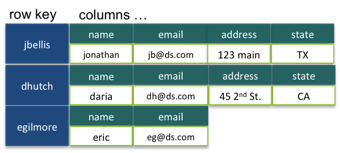
\includegraphics[scale=0.95]{images/static_column_family}
\caption{Schéma datového modelu v Column Family}
\label{fig:vnodes}
\end{figure}

\begin{figure}[!h]
\centering
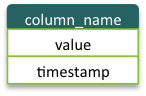
\includegraphics[scale=1.5]{images/column}
\caption{Schéma datového modelu Column}
\label{fig:vnodes}
\end{figure}

\section{CQL}
Přestože bylo v předchozí sekci řečeno, že Thrift je zastaralý a CQL je doporučená cesta jak se dotazovat nad daty, datový model je stále velmi důležitý a je potřeba mu rozumět, abychom dokázali náš model navrhnout funkčně a efektivně. Thrift nám tento model přímo odhaluje a CQL je pouze abstrakcí, která nám dovoluje pracovat s daty obdobně, jako jsme zvyklí v relačním světě s tím rozdílem, že si poté dotazy převede na dotazy nad zmíněným interním datovým modelem. 

CQL je dotazovací jazyk podobný SQL, přes který lze vytvářet datové struktury – tabulky – které mají stejný formát jako tabulky relační, avšak na pozadí se struktury i dotazy nad nimi převedou na datový model popsaný v předchozí kapitole. CQL neumožňuje žádný příkaz z \uv{rodiny} JOIN. Přestože by se mohlo zdát, že pevná struktura nás omezuje oproti předchozím návrhům, opak je pravdou. Pomocí CQL jsme schopni vymodelovat data o různých hodnotách. Konkrétní příklady budou popsány v následující kapitole. 

\newpage

\begin{lstlisting}[caption={Tvorba jednoduché tabulky pomocí CQL},label=CQL1]
CREATE TABLE songs (
  id uuid PRIMARY KEY,
  title text,
  album text,
  artist text,
  data blob
 );
\end{lstlisting}

Jak je z kódu \ref{CQL1} patrné, syntaxe jazyka CQL se opravdu od SQL příliš neliší. Jazyk má různé funkce, ale také určitá omezení, jejichž kompletní popsání by vydalo na samostatnou práci. Jen krátce bych chtěl upozornit, že jazyk podporuje indexy na sloupcích, ale také datové kolekce. Nejdůležitější funkce a omezení budou rozebrány v rámci případů užití v následující kapitole. Na závěr přikládám tabulku převodů interních typů na typy využívané v jazyce CQL.

\begin{table}[h]

    \begin{tabular}{|l|l|l|}
    \hline
    Internal Type     & CQL Name      & Description                                    \\ \hline
    BytesType         & blob          & Arbitrary hexadecimal bytes (no validation)    \\ \hline
    AsciiType         & ascii         & US-ASCII character string                      \\ \hline
    UTF8Type          & text, varchar & UTF-8 encoded string                           \\ \hline
    IntegerType       & varint        & Arbitrary-precision integer                    \\ \hline
    Int32Type         & int           & 4-byte integer                                 \\ \hline
    LongType          & bigint        & 8-byte long                                    \\ \hline
    UUIDType          & uuid          & Type 1 or type 4 UUID                          \\ \hline
    TimeUUIDType      & timeuuid      & Type 1 UUID only (CQL3)                        \\ \hline
    DateType          & timestamp     & Date plus time, encoded as 8 bytes since epoch \\ \hline
    BooleanType       & boolean       & true or false                                  \\ \hline
    FloatType         & float         & 4-byte floating point                          \\ \hline
    DoubleType        & double        & 8-byte floating point                          \\ \hline
    DecimalType       & decimal       & Variable-precision decimal                     \\ \hline
    CounterColumnType & counter       & Distributed counter value (8-byte long)        \\ \hline
    \end{tabular}
    \caption {Interní Datové typy}
   \label{datatypes}
\end{table}


\chapter{Vhodné případy užití}
Některé vhodné případy použití byly definovány v~průběhu textu. V~této sekci se zaměřím na obecné příklady použití, respektive na modelování základních situací. Poté shrnu zajímavé případy použití, které světově významné firmy používající Cassandru prezentovaly na Cassandra Summitu 2013 v~Londýně, kterého jsem se zúčastnil. V~poslední části této kapitoly se budu věnovat případům využití, které jsem sám použil ve své praxi a nebo navrhoval v~analýzách projektů. 

\section{Obecné modelování}

\subsection{Jednoduché struktury s~nesloženým primárním klíčem (Statické tabulky)}

Pokud struktura dat nevyžaduje žádné složité operace a dotazy a vystačíme si s~modelem, kde klíč je tvořen jedním sloupcem (tedy například pouze nějaký hash), můžeme použít jednoduchou definici tabulky jako v~\ref{CQL1}. Z~této tabulky pak jednoduše data čteme i zapisujeme tak, jak jsme zvyklí z~klasického SQL.

\subsection{Struktury se složeným primárním klíčem (Dynamické tabulky)}

Dříve než popíšeme, jakým způsobem je možné vytvářet dynamické tabulky, je potřeba vysvětlit, jak Cassandra zachází se skládáním primárních klíčů

\subsubsection*{Složené klíče}
V~Cassandře můžeme skládat klíče ze 2 části (ty mohou být tvořeny jedním sloupcem nebo opět složenými sloupci). První část klíče se nazývá \uv{Partition Key} a určuje, z~čeho se bude skládat interní primární klíč, tedy ten, co se hashuje a následně distribuuje po clusteru. Druhá část klíče se nazývá \uv{Clustering Key}, který automaticky na daných sloupcích vytváří index a řadí data dle těchto sloupců. Interně slouží tyto sloupce jako prefix v~názvech ostatních sloupců a fragmentujeme podle nich data uvnitř jedné řádky. 

\begin{lstlisting}[caption={Ukázka složených klíčů},label=CQL2]
CREATE TABLE Cats (
  block_id uuid,
  breed text,
  color text,
  short_hair boolean,
  PRIMARY KEY ((block_id, breed), color, short_hair)
);
\end{lstlisting}

Příklad \ref{CQL2} ukazuje, že Partition Key je složený ze sloupců \emph{block\_id} a  \emph{breed} a clustering sloupce jsou \emph{color} a \emph{short\_hair}. Cassandra uloží data, která mají stejný \emph{block\_id}, ale jiný \emph{breed}, na jiný uzel než data, která mají hodnoty těchto sloupců stejné.  


\subsubsection*{Časosběrné události 1}
Ideálním příkladem na ilustraci toho, jak se používají složené klíče (respektive implementace dynamických tabulek), tedy využití vlastnosti Cassandry, že v~Column Family nemusí mít pevný formát sloupců, jsou časosběrné události. Ukládáme různé hodnoty v~čase na různých místech nebo pro různé uživatele. Ukázkový příklad sbírá data na meteorologických stanicích a ukládá aktuální teplotu pro daný čas.

\begin{lstlisting}[caption={Dynamická tabulka 1},label=CQL3]
CREATE TABLE temperature (
   weatherstation_id text,
   event_time timestamp,
   temperature text,
   PRIMARY KEY (weatherstation_id,event_time)
);
\end{lstlisting}

Jako primární klíč jsme zvolili id stanice, které bude tvořit také interní klíč pro Cassandru a čas události, což bude název sloupce, který bude mít jako hodnotu aktuální teplotu. Sloupce se interně budou automaticky řadit podle času. Interně tedy bude následující tabulka vypadat následovně: 

\begin{figure}[h]
\centering
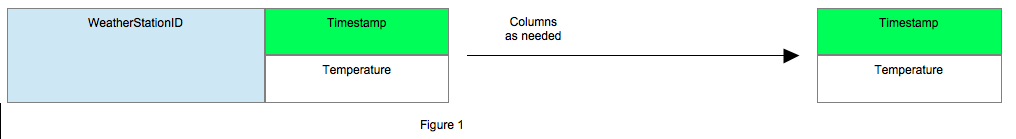
\includegraphics[scale=0.4]{images/timeseries1}
\caption{Interní reprezentace dat tabulky \ref{CQL3}}
\label{fig:timeseries1}
\end{figure}

Jak je z~obrázku \ref{timeseries1} patrné, tímto formátem využíváme zmíněnou výhodu o~odlišné struktuře řádek v~Column Family. Každá meteostanice má vlastní řádek a sloupce tvoří časové razítko, kdy byla naměřena daná hodnota. Časová razítka mohou být samozřejmě pro každou stanici jiná a tudíž bude mít i každá řádka odlišné sloupce. Takto můžeme data jednoduše vkládat a dotazovat se nad nimi. V~případě časosběrných událostí máme ovšem jednu nevýhodu. Jsme limitování maximálním počtem sloupců, kterých je sice asi 2 miliardy, ale pokud uvážíme, že bysme data měřili každou milisekundu, dojdou nám sloupce dřív než za měsíc.  

\subsubsection*{Časosběrné události 2}
U~předchozího řešení jsme narazili na problém, kdy nám mohou dojít sloupce pro danou řádku. Řešení tohoto problému je celkem jednoduché, použijeme při navrhování modelu vzor \uv{Rozdělení řádky}, kdy první část primárního klíče (Partition Key) složíme ze dvou sloupců stejně jako v~ukázce \ref{CQL2}.


\begin{lstlisting}[caption={Dynamická tabulka 2},label=CQL4]
CREATE TABLE temperature_by_day (
   weatherstation_id text,
   date text,
   event_time timestamp,
   temperature text,
   PRIMARY KEY ((weatherstation_id,date),event_time)
);
\end{lstlisting}

Tabulku jsme upravili tak, že jsme přidali sloupec \emph{datum}, který zároveň tvoří Partition Key. Data se budou ukládat pro každou stanici a každý den do samostatné řádky, čímž je limit 2 miliardy sloupců vyřešen, protože v~našem případě počítáme, že jedna stanice nebude denně provádět více než 2 miliardy měření. Interně to bude vypadat tak, že spojíme id stanice a datum, z~této hodnoty se vytvoří interní row key a ten rozhodne, na který uzel se data uloží. Schéma se změní následovně: 

\begin{figure}[h]
\centering
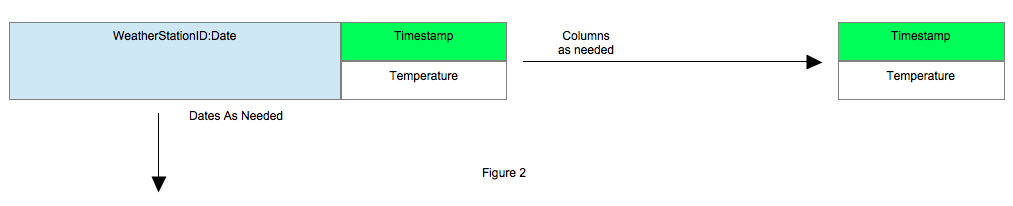
\includegraphics[scale=0.4]{images/timeseries2}
\caption{Interní reprezentace dat tabulky \ref{CQL4}}
\label{fig:timeseries1}
\end{figure}

Jak je vidět z~předchozího příkladu, návrh a struktura dat se musí opravdu dobře rozmyslet předem, případné chyby v~návrhu (např. opomenutí limitů) se poté řeší velice nepříjemně. Komplikovanější návrh nezabere implementačně moc času navíc a bude fungovat pořád.


\subsection{Mixování statických a dynamických tabulek}
Cassandra nativně umožňuje i mixování předchozích vzorů. Například máme dynamický prvek \emph{tag}, který přiřazujeme k~uživateli, jehož ostatní sloupce jako jméno, adresa atd. jsou obyčejná statická tabulka. Cassandra takovýto návrh řeší nativně pomocí kolekcí. Kolekce jsou datový typ v~CQL, který umožňuje mít v~jednom sloupci více hodnot a pracovat s~nimi. Cassandra nabízí následující typy kolekcí:

\begin{itemize}
\item Set - ADT množina
\item List - ADT seznam
\item Map - ADT tabulka
\end{itemize}

Každý typ kolekce obsahuje odpovídající operace a chování, jaké se dá očekávat u~těchto abstraktních datových typů. Kolekce se dají použít kdykoliv, kdy chceme do statického modelu přidávat konečný (dopředu neznámý) počet malých hodnot. Kolekce mají následující omezení: 

\begin{itemize}
\item Maximální množství objektů v~kolekci je 64 000.
\item Maximální velikost objektu v~kolekci je 64Kb
\end{itemize}

\section{Jak Cassandru používají významné firmy a služby}

V~této sekci bych rád popsal několik reálných případu užití Cassandry ve všeobecně známých firmách či službách. Některé z~těchto případů užití byly demonstrovány na Cassandra Summit 2013, kterého jsem se v~rámci tvorby této práce zúčastnil a s~některými techniky daných firem jsem o~implementaci Cassandry v~jejich řešení hovořil. 

\subsection{Spotify a hudební seznamy}
Spotify je jedním z~největších hráčů na trhu online přehrávání hudby. Spotify však Cassandru nevyužívá k~ukládání informací o~skladbách či snad k~ukládání skladeb samotných, jak by se mohlo na první pohled zdát. Ve Spotify používají Cassandru k~ukládání seznamů skladeb. Takovýchto seznamů mají více než 1 miliardu a musejí řešit několik zádrhelů ohledně jejich kolaborativních úprav. Seznamy skladeb totiž mohou být editovatelné více uživateli nebo jedním uživatelem z~více míst a nebo dokonce je možné provádět jejich úpravy v~offline režimu. 

Ve Spotify si s~touto výzvou poradili výborně. Každý playlist je vlastně verzovaný objekt s~jednoduchými operacemi: \emph{MOV} posune skladbu z~nějakého místa na jiné, \emph{ADD} na vybrané místo skladbu vloží, \emph{DEL} vymaže skladbu ze seznamu. Každou takovouto operaci zaznamenávají se speciálním časovým razítkem a odkazem na předchůdce tohoto otce. Dále si v~jiné CF ukládají odkaz na takzvaný \emph{HEAD}, tedy poslední operaci. Díky souběžným změnám může být těchto hlaviček několik, což vede k~rozvětvení playlistu v~určitém bodě. Pomocí algoritmů operačních transformací dokáží z~libovolného místa seznam zreprodukovat a dokonce provést sjednocení rozdělených větví. Cassandra je tedy vhodná k~použití kdykoliv, kdy potřebujeme uložit velké množství jakkoliv verzovaných objektů. 

\subsection{Netflix}
Netflix patří mezi největší hráče na poli streamování video obsahu. Přestože se jedná v~principu o~podobnou službu jako Spotify, v~Netflixu využívají Cassandru pro ukládání úplně jiných dat. A~to téměř všech dat, které mají k~dispozici. Netflix má po celém světě přes 30 milionů aktivních uživatelů a do Cassandry ukládají informace o~uživatelích, metadata o~veškerém video obsahu nebo dokonce statistiky. Zajímavostí je, že Netflix nemá žádnou vlastní infrastrukturu a veškeré servery hostují přes službu Amazon AWS. Netflix je také jedním z~velkých přispěvatelů do zdrojových kódů Cassandry a to převážně právě do sekce věnující se nasazení a správě Cassandra clusteru na této službu od Amazonu. Tento případ užití by měl zviditelnit výhody ukládání plochých databázových struktur napříč několika datacentry po celém světě. 

\subsection{Ebay} 
Ebay je největší internetová aukční síň, která má desítky milionů uživatelů. Cassandru využívá na několik svých služeb. První z~nich je unikátní doporučovací systém. Každý uživatel prochází desítky položek při hledání určitého zboží a na základě toho, na které položky klikl nebo naopak neklikl, je mu doporučováno další zboží. Ebay ukládá veškeré tyto události formou grafu, který znázorňuje uživatele, nabízené zboží a vztahy mezi nimi. Díky tomuto systému může Ebay svým uživatelům nabízet stále přesnější výsledky. 

Ebay využívá Cassandru také na zpracovávání sociálních dat, jako jsou například zobrazení, přání a oblíbené položky. Tyto hodnoty pro jednotlivé produkty vždy napočítá pomocí MapReduce. 

Poslední případ, na který v~Ebayi Cassandru používají, jsou v~podstatě jakékoliv časosběrné události. Například:
\begin{itemize}
\item Mobilní notifikace jejich logování a sledování
\item Sledování dat pro následné odhalování podvodů
\item Analýza serverových logů a analytických dat
\end{itemize}

Využití Cassandry v~Ebayi ukazuje další stránky využitelnosti této databáze (například výše zmiňované časosběrné požadavky). Ebay považuje Cassandru za přínos hlavně z~hlediska škálovatelnosti a množství zápisů, které lze souběžně provádět. Ebay totiž za den provede do Cassandry přibližně 6 miliard zápisů.\cite{ebay} Ebay, kvůli plné integraci s~Hadoopem, navíc používá ve všech svých clusterech DataStax Enterprise, přes který provádí MapReduce. Schéma Ebay Cassandra clusteru vypadá přibližně následovně:

\begin{figure}[h]
\centering
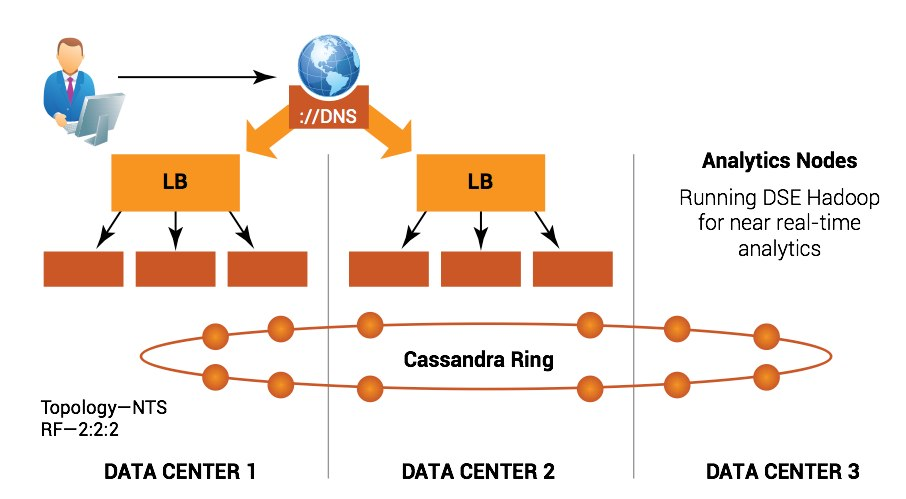
\includegraphics[scale=0.4]{images/ebay}
\caption{zdroj:  Cassandra at Ebay \cite{ebay}}
\label{fig:timeseries1}
\end{figure}

\subsection{Finn.no}
Finn.no je největší norský webový server. Týdně přivítá 3,5 milionu návštěvníků v~zemi, která má 5 milionů obyvatel. Jedná se o~inzertní portál, přes který lidé nabízejí či poptávají reality, pracovní pozice, věci na prodej, automobily, dovolené a služby. Na většinu z~těchto oblastí má Finn.no v~zemi \uv{monopol}. Tento inzertní server Cassandru opět využívá na několik způsobů. Prvním je ohodnocení každé nabídky, která přijde a její prověření, zda se nejedná o~podvod. V~případě podezření je taková nabídka přeposlána k~manuální kontrole. Dále Cassandru využívají na implementaci zpráv mezi uživateli, což je vlastně originální případ užití a důvod vzniku Cassandry kdysi v~kancelářích Facebooku. Cassandru zde využívají i na uchovávání uživatelovy historie hledání, kdy se uchovávají jednotlivé informace o~každém hledání a uživatel si může v~profilu prohlédnout, co hledal. V~tomto případě se návrháři rozhodli, že jim stačí uchovávat data pouze za posledních 6 měsíců, a proto využívají expirující sloupce, které po 6 měsících automaticky zmizí. Posledním případem využití je podobné sčítání zobrazení nebo přidání inzerátu do sledovaných jako na Ebay. Jednou za hodinu se spustí Hadoop Job, který pomocí MapReduce namapuje potřebné údaje, posčítá je a následně uloží zpět do databáze.

Zajímavostí na implementaci Finn.no je, že většina firem používá více menších strojů. Ve Finn.no mají pouze 6 uzlů s~velice výkonným hardwarem. Důvodem je lokalita dat, která pro ně má mnohem větší cenu než drobné blokující IO operace. 

\section{Ostatní navržené případy užití}

V~této sekci bych se na závěr kapitoly chtěl zaměřit na případy užití, se kterými jsem přišel do styku v~reálném prostředí nebo je teoreticky navrhoval pro nerealizované či věděcké projekty. 

\section{Analýza access logů}
První z~těchto zajímavých případů užití se týká analýzy access logů. Dostal jsem za úkol navrhnout řešení, které by umožnilo velké nadnárodní společnosti s~pobočkami po celém světě a více než 20 000 zaměstnanci monitorovat, jaké weby její zaměstnanci navštěvují v~pracovní době. Na základě těchto dat poté tvořit grafy a reporty pro konkrétní uživatele nebo oddělení. Součástí analýzy řešení byl i prototyp vybraného řešení. Seznam požadavků byl následující: 

\begin{itemize}
\item Možnost stahování či uploadu dat z~access logů do systému
\item Pro konkrétního uživatele či oddělení vyrobit report obsahující:
\begin{itemize}
\item Zobrazení dat za vybrané časové období (1 týden až 6 měsíců zpět) 
\item Zobrazení navštívených stránek s~absolutním číslem přístupů a procentuálním poměrem. 
\item Zohlednění příznaku firewallu o~statusu požadavku (OK, Podezřelý, Nepřípustný)  
\end{itemize}
\item Data uchovávat pouze po dobu 6 měsíců 
\item Data musí být přístupná ihned, avšak klidně s~denním zpožděním (logy se nestahují z~celého světa současně)
\end{itemize}

Po sběru požadavků jsem ihned identifikoval, že toto je přímo ukázkový příklad pro využití Cassandry. 

Tento případ užití jsem shledal natolik zajímavý a to jak z~hlediska možností implementace, praktického přínosu a významnosti, že jsem po domluvě s~vedoucím práce tento případ využití použil i v~praktické části a závěrečné části této práce, kde ho dopodrobna rozeberu.

\section{Obrázkové servery}
Dalším zajímavým případem využití, se kterým jsem se setkal, je i příklad užití, kde se čtení provádí mnohonásobně častěji než zápis. Takovým způsobem funguje obrázkový server. V~dnešní době mobilních zařižení je naprosto běžné, že potřebujeme mít obrázek v~několika velikostech. Vzhledem k~rostoucímu počtu různorodých zařízení vznikají potřeby pro nová a nová rozlišení. Na toto můžeme využít Cassandřinu vlastnost nepevného schématu. Pro každý obrázek uložíme originální velikost včetně metadat a při dotazu na něj příslušný obrázek vytáhneme z~databáze. Samozřejmě by celé řešení bylo vhodné doplnit o~nějakou vrstvu cachování. Tento use case je velice praktický a komplexní, jelikož závisí na ostatním nedatabázovém softwaru, a proto jsme se po konzultaci s~vedoucím práce rozhodli obrázek zařadit. Podobným způsobem uchovával své obrázky například Facebook, než napsal vlastní nízkoúrovňový systém na správu fotografií. 

\section{Sběr a vyhodnocení transakčních událostí}
V~maloobchodě je běžné zjišťovat oblíbenost produktů a hledat vazby mezi jednotlivými předměty a uživateli ukládáním všech transakcí a jejich následným přiřazováním ke konkrétním uživatelům (například v~e-shopu nebo pomocí věrnostní karty). Správnou manipulací s~daty jsme schopni vymodelovat například následující grafy:

\begin{itemize}
\item Uživatelé, co zakoupili produkt X, také zakoupili tyto produkty.
\item Graf uživatelů, kde hrany reprezentují vazbu alespoň jednoho společně zakoupeného předmětu. Ohodnocení hrany znamená počet takovýchto předmětů. 
\end{itemize} 
Předchozí grafy lze také upravovat změnou množiny předmětů a sledovat změny na základě určité skupiny předmětů. Takovéto grafy dokáží odhalit vazby mezi předměty, ale také vazby a podobnost mezi uživateli a předpovídat jejich další aktivitu. 
\newpage
\section{Hledání korelací}
Pokud máme dostatek dat, můžeme se mezi dvěma veličinami snažit o~hledání kovariance, respektive korelačního koeficientu. Veličinou myslíme hodnotu dat v~čase. Například každý den ukládáme, kolik jsme prodali kusů kterého zboží, jaká je teplota, jaký je aktuální kurz měny atd. Můžeme pak jednoduše hledat spojitosti například mezi počasím a počtem prodaného zboží nebo vztah 2 různých prodávaných artiklů mezi sebou. Pro obchodníky jsou poté tato data velice důležitá, protože jim pomáhají lépe pochopit myšlení svých zákazníků, předpovídat jejich chování a také lépe plánovat provoz svého podnikání. Tento případ užití si ve zjednodušené podobě popíšeme i v~následující kapitole. 

\section{Podpora v~plně distribuované síti}
Ing. Josef Gattermayer vede výzkumný projekt zabývající se plně distribuovaným systémem na rozesílání zpráv mezi uzly. Tento problém se zatím řeší pouze v~teoretické rovině a jedním z~problémů, který je potřeba vyřešit, je notifikování uzlů, které byly offline, že na ně někde čeká zpráva. 

V~tomto ohledu jsem se nechal inspirovat vlastností, kterou Cassandra používá při zapisování, a tou je konkrétně \uv{Hinted Handoff}, který byl popsán v~předchozích kapitolách. Tento návrh předpokládá, že cluster je (z~hlediska infrastruktury jednotlivých uzlů a služeb na nich běžících) nehomogenní. Návrh spočívá v~tom, že přestože by si všechny uzly byly rovny po stránce komunikační, některé uzly by byly zároveň uzly perzistentními, které by ukládaly informace například do Cassandry. Těmito perzistentními uzly by zpravidla měly být nějaké serverové stanice. U~ostatních komunikačních uzlů se nemusíme omezovat pouze na servery a můžeme počítat i se zařízeními, jako jsou mobilní telefony či přenosné počítače. Komunikační proces by v~případě neúspěšného doručení zprávy byl následující: 

\begin{enumerate}
\item Uzel A~vyšle zprávu pro uzel B
\item Uzel C zjistí nedoručitelnost, protože uzel B je nedostupný
\item Uzel C kontaktuje jeden z~perzistentních uzlů a zprávu do něj uloží s~určitou dobou platnosti. 
\end{enumerate}

Při změně stavu uzlu B zpět online se provedou následující operace:

\begin{enumerate}
\item Uzel B kontaktuje kterýkoliv perzistentní uzel s~dotazem, zdali pro něj má nějaké nedoručené zprávy
\item Perzistentní uzel pošle pro něj uchovanou zprávu uzlu B
\item Perzistentní uzel zašle zprávu o~doručení uzlu
A~\end{enumerate}


V~případě, že chceme striktně dodržovat distribuovanost informací, nebudeme na perzistentní server ukládat zprávy jako takové, ale budeme ukládat pouze takzvané hinty a operace budou probíhat následovně: 

\begin{enumerate}
\item Uzel A~vyšle zprávu pro uzel B
\item Uzel C zjistí nedoručitelnost, protože uzel B je offline
\item Uzel C zkontaktuje zpět uzel A~s~informací, že zprávu nelze odeslat
\item Uzel A~si zprávu uloží a zkontaktuje perzistentní server, aby uložil hint pro uzel B

\end{enumerate}

Při změně stavu uzlu B zpět online se provedou následující operace:

\begin{enumerate}
\item Uzel B kontaktuje kterýkoliv perzistentní uzel s~dotazem, zdali pro něj má nějaké nedoručené zprávy
\item Perzistentní uzel pošle uzlu B hint o~tom, že uzel A~pro něj má zprávu
\item Uzel C zašle uzlu A~požadavek na znovuposlání zprávy
\end{enumerate}


V~obou předchozích scénářích předpokládáme, že uzel B se stane nedostupným až po odeslání zprávy. Před odesláním zprávy si tuto informaci může zjistit uzel A~sám a provede tudíž operace, jako kdyby byl uzlem C, aniž by zprávu někam posílal. Ve druhé variantě je potřeba ošetřit problém cyklických hintů, pokud uzly budou navzájem střídavě nedostupné a pro jednu zprávu by mohlo být uloženo nekonečně mnoho hintů. Pro daný pár uzlů nám vždy stačí mít uložen právě jeden hint pro daný směr požadavku. Tento případ užití je pouze teoretický a měl by demonstrovat možnost využití distribuovaného systému, jako je Cassandra, v~jiných distribuovaných systémech jako úložiště nebo monitorovací prvek tohoto systému. 


\chapter{Popis implementace vybraných případů užití}
V~předchozí kapitole jsem popsal několik různých druhů užití Cassandry v~reálných podmínkách. Vzhledem k~zadání této práce jsem (po konzultaci s~jejím vedoucím) vybral několik jednoduchých a rozdílných případů, které budou sloužit jako podklady pro přípravu cvičení a laboratoří nově připravovaného předmětu na ČVUT.

\section{Testovací prostředí}
Součástí zadání bylo vypracovat tyto případy užití na školní infrastruktuře. Vzhledem ke komplikované instalaci a správě veškerého potřebného softwaru bylo z~hlediska efektivity práce od této myšlenky upuštěno. Fakulta vlastní experimentální výpočetní cluster a Tomáš Bartoň, kterému bych tímto chtěl poděkovat, mi nabídl řešení, které se zprvu zdálo dostačující, ale vzhledem ke komplikacím jsme i od tohoto řešení museli upustit. Finální implementace tedy proběhla na clusteru vytvořeném z~virtuálních strojů na jednom fyzickém počítači pomoci XENu. Pro Ing. Gattermayera, který předmět připravuje, jsem připravil XEN obraz, díky kterému lze vytvořit nový uzel a spustit na něm Cassandru. Toto řešení se ukázalo i pro garanta předmětu jako nejvhodnější a nejjednodušší. 

\section{Implementace access log analyzéru}
Jak bylo zmíněno v~předchozí kapitole, dostal jsem za úkol vypracovat analýzu a prototyp řešení pro nadnárodní německou firmu zaměstnávající více než 20 000 lidí po celém světě. Tito lidé se z~firemní infrastruktury připojují do internetu a firma chce monitorovat návštěvnost stránek jednotlivých uživatelů a oddělení pro různá časová období, která však nejsou delší než 6 měsíců a na základě různých kriterií generovat online reporty. Tento zdánlivě jednoduchý problém v~sobě ve skutečnosti skrývá několik netriviálních úkolů. Především je to množství dat, které je potřeba zpracovat. Pokud bychom zpracovávali data sekvenčně, tak bychom museli procházet přibližně 1860 GB systémových logů, což bychom rozhodně v~žádné relační databázi nemohli provést v~rozumném čase. Data dostáváme inkrementálně každý den (vždy za předchozí den) a to v~několika dávkách z~různých serverů po celém světě. 


\subsection{Návrh řešení pro ukládání všech logů}
Rozhodl jsem se tedy, že budu data ukládat do tabulky v~Cassandře. Všechna data budu zapisovat s~atributem TTL tak, aby se za půl roku automaticky smazala. Strukturu tabulky jsem navrhl následovně: 

\begin{lstlisting}[caption={Návrh tabulky pro ukládání všech logů},label=LogTable]
CREATE TABLE accesslog_ks.logs ( 
user text,
date timestamp,
webpage text,
severity text,
PRIMARY KEY (user,date) 
);
\end{lstlisting}

Sloupec \emph{severity} znázorňuje \uv{nebezpečnost} dotazu, tak jak ji vyhodnotil proxy server. Tento údaj byl součástí analýzy a celý příklad značně komplikuje, jak bude vysvětleno níže. Jako primární klíč jsem zvolil návrhový vzor pro časosběrné údaje, tedy uživatele a časové razítko. Pro zjednodušení tohoto příkladu předpokládáme, že uživatel v~jednu vteřinu nepřistoupí na více webových stránek. V~reálném světě by bylo dobré do klíče přidat i webovou stránku či zpřesnit časové razítko až na milisekundy. 

\subsection{Naivní řešení}
Prvním řešením, jak získat data pro reporty, je dotazování se přímo nad tabulkou logů. Nápad by se mohl zdát naprosto špatný, ale opak je pravdou. Jak dokládá následující tabulka, pokud by nám šlo o~jedno konkrétní datum, je přístup do databáze velice rychlý i přes obrovské množství záznamů a prokazuje se, jak mocná Cassandra je. Čas nutný na přístup ke všem datům je na toto množství záznamů také výborný, avšak pro větší záznamy bychom již nedosahovali časů vhodných k~online reportu. Navíc v~této struktuře nemůžeme jednoduše třídit data a veškeré řazení a vyhodnocování bychom museli následně provádět v~kódu, což by bylo velice zdlouhavé a neefektivní. Nemluvě o~situaci, kdy bychom se dotazovali na různá oddělení a museli bychom provádět dotazů několik. Data v~tabulce neodpovídají reálnému provozu, všechny uzly se nachází na jednom ne příliš výkonném počítači s~jedním diskem, takže IO operace jsou velice limitované a následná komunikace s~testovacím prostředím probíhá přes lokální síť. Reálné hodnoty by byly mnohonásobně nižší, cílem je poukázat na rozdíl hodnot v~různých situacích.    

\begin{table}[h]
%\begin{tabularx}{\textwidth}{ |l|l|l|l||| }

    \begin{tabular}{|l|l|l|l|l|}
    \hline
    \begin{tabular}{@{}c@{}}Počet \\záznamů \end{tabular} &  \begin{tabular}{@{}c@{}}Přibližný počet \\záznamů na uživatele \end{tabular} &  Vše [ms] & 1/3 [ms] & 1 den [ms] \\ \hline
    1000          & 200                                  & 160                  & 40                 & 20               \\ \hline
    11000         & 2000                                 & 600                  & 300                & 60               \\ \hline
    111000        & 20000                                & 3887                 & 1243               & 70               \\ \hline
    \end{tabular}
    \caption {Měření dotazování nad tabulkou logů}
\end{table}

\subsection{MapReduce 1}
Samozřejmě existuje ještě lepší řešení, kterým je MapReduce. Data zredukujeme a uložíme do pomocné tabulky. Nejdříve projdeme schéma výsledné tabulky a následně si ukážeme mapovací a redukční funkci.

\begin{lstlisting}[caption={Tabulka pro ukládání reportů},label=ReportTable]
CREATE TABLE accesslog_ks.reports ( 
user text,
webpage text,
date timestamp,
severity text,
count int,
PRIMARY KEY ((user,severity),date,webpage) 
);
\end{lstlisting}

Formát tabulky je zde téměř stejný jako v~tabulce s~logy (až na pár výjimek). Sloupec \emph{date} nyní neoznačuje přesné časové razítko, nýbrž pouze označení data bez času. Navíc zde přibyl sloupec \emph{count}, který obsahuje informaci o~celkovém počtu navštívení dané webové stránky pro tento den. Velice důležité je zde složení primárního klíče, které určuje, jak se data budou ukládat a řadit uvnitř databáze. Důvody k~výše uvedené skladbě klíče jsou následující. 

Kvůli jednoznačnému určení potřebujeme, aby klíč obsahoval všechny výše zmíněné atributy. Abychom se mohli dotazovat na konkrétní uživatele, musí být uživatel Partition Key, respektive jeho první částí. Abychom se mohli dotazovat na všechny nebo pouze na vybrané úrovně závažnosti, musí být uvedeny jako druhá část partition klíče. Tato volba je přirozená, jelikož hodnota \emph{severity} nabývá konečného počtu předem známých hodnot, a proto nebudeme tolik fragmentovat. Kdybychom \emph{severity} a \emph{user} prohodili, mohli bychom se sice ptát na více uživatelů, ale pouze na jeden konkrétní stupeň závažnosti, což je vzhledem k~našemu zadaní nelogické a neoptimální.

Po partition klíči následují další části primárního klíče, jako je datum, protože podle něj se budou výsledky uvnitř partition řadit, což je přesně to, co chceme a navíc kdybychom \emph{date} a \emph{webpage} prohodili, museli bychom se dotazovat na konkrétní webovou stránku, abychom se vůbec mohli ptát na datum, což je vzhledem k~funkcím aplikace nesmyslné. Jak je vidět, pořadí sloupců tvořící primární klíč je velice důležité! Takto složený klíč je pro námi zadaný příklad jediné správné a optimální řešení.

\subsubsection{Mapovací funkce}
Mapovací funkce je v~tomto případě velice jednoduchá. Musíme vytvořit univerzální schéma klíče, abychom mohli sečíst návštěvy v~daný den. Proto potřebujeme datum \uv{normalizovat}. V~případě data nám stačí jej oříznout pouze na rok, měsíc a den. Čas požadavku nás nezajímá. Z~informací \emph{normalizované datum}, \emph{adresa}, \emph{uživatel} a \emph{úroveň závažnosti} vytvoříme klíč, ke kterému přiřadíme hodnotu 1, protože se jedná o~jednu návštěvu dané webové stránky v~jeden den konkrétním uživatelem. 

\subsubsection{Redukční funkce}
Redukcí pro každý klíč provedeme sumu hodnot, tedy počtu navštívení a výsledek zapíšeme do výše uvedené tabulky s~výše popsaným primárním klíčem, který se rovná stejnému klíči, který jsme vytvořili v~mapperu. 

\subsection{MapReduce 2}
V~předchozím případě jsme viděli, jak napsat MapReduce job pomocí vlastního algoritmu, tedy nadefinování mapovací a redukční funkce. V~tomto případě to bylo relativně jednoduché a moc práce nám to nedalo. Přesto je potřeba napsat několik tříd a vše správně zkompilovat a poté spustit. V~druhém způsobu popíši, jak používat dotazovací jazyk Hive, který dotazy sám přeloží do MapReduce kódu, který spustí a vrátí výsledek. Tabulku na ukládání výsledků MapReduce jobů ponecháme stejnou jako v~prvním případě, výsledek je totiž stejný. V~jazyce Hive nám k~předchozímu výsledku stačí pouze takovýto dotaz:

\begin{lstlisting}[caption={Tabulka pro ukládání reportů},label=Hive1]
select 
to_date(cast(logs.date as bigint)) as trimdate,
logs.user,
logs.webpage,
logs.severity, 
count(*) as count
from logs 
group by logs.webpage, logs.severity, logs.user,
to_date(cast(logs.date as bigint));
\end{lstlisting}

Tento dotaz vypadá složitě, ale je to jednoduchý SQL dotaz, který je programátorům využívajícím SQL dobře srozumitelný. Jediná komplikovanější věc je funkce, která nám ořeže datum. Výsledkem tohoto dotazu jsou spočítané návštěvy stránek pro každý den pro všechny uživatele. Tento dotaz spustíme klasicky přes Hive JDBC konektor a jeho výsledky přes Cassandra JDBC konektor zapíšeme. Výsledek je stejný jako v~předchozím případě s~minimem psaní kódu, za cenu trochu delší doby běhu, která jde na vrub generování MapReduce jobu. 

Hive experimentálně podporuje i vkládání do Cassandry přes externí tabulku, kterou když vytvoříme, tak před dotaz \ref{hive1} vložíme příkaz \emph{INSERT INTO table}, kde \emph{table} je název naší externí tabulky. Kód pro vytvoření a namapování tabulky vypadá následovně: 

\begin{lstlisting}[caption={Vytvoření externí tabulky napojené na tabulku v~CQL},label=Hive2]
CREATE EXTERNAL TABLE hivereports (user string, webpage string,date timestamp, severity string, count int)
        STORED BY 'org.apache.hadoop.hive.cassandra.cql3.CqlStorageHandler'
        TBLPROPERTIES ( "cassandra.ks.name" = "accesslog_ks",
        "cassandra.cf.name" = "reports",
        "cassandra.ks.repfactor" = "2",
        "cassandra.ks.strategy" =
        "org.apache.cassandra.locator.SimpleStrategy");
    
ALTER TABLE hivereports SET TBLPROPERTIES ('cql3.output.query' = 'update accesslog_ks.reports set count = ? where user = ?  and webpage = ? and severity =?');
    
ALTER TABLE hivereports SET SERDEPROPERTIES ('cql3.update.columns' = 'user,webpage,date,severity,count');
\end{lstlisting}

Tento postup je ovšem vskutku experimentální a zatím nefunguje pro všechny případy, a proto se jeho užití zatím obecně nedoporučuje. V~případě napojení přes externí tabulku by nám tedy stačil jediný krátký dotaz a data by se nám uložila stejně jako v~prvním případě. Nevýhodou ovšem zůstává, že takto nemůžeme použít TTL funkci při zápisu do Cassandry.

\subsection{Optimalizace}
Jednou možnou optimalizací je omezení zadání na předdefinované celky času. Například jeden den zpět, minulý týden nebo minulý měsíc. Tedy, že výběr data nebude libovolný, čímž bychom snížili množství zápisů do tabulky reportů a výběr těchto dat by byl rychlejší. 

Druhou a poněkud zásadnější optimalizací je, že v~předchozích příkladech řadíme vždy z~celé množiny dat. Tomu můžeme předejít tím, že budeme MapReduce provádět pouze nad dnešními daty. Vzhledem k~pravidelnému inkrementálnímu přírůstku dat je tato optimalizace vhodná, protože nebudeme zbytečně pracovat s~daty, která už máme jednou vypočítaná. 

\subsection{Skupiny Oddělení}
Součástí zadání je, že uživatel může chtít zobrazit souhrnný report pro celé oddělení. V~současné variantě bychom museli pro každého uživatele z~oddělení udělat samostatný dotaz a výsledky spočítat. Takové řešení je samozřejmě neefektivní. Pomůžeme si jednoduchým trikem. Tabulku s~logy rozšíříme o~sloupec s~informací o~oddělení a vytvoříme druhý MapReduce nebo Hive dotaz, který nebude brát v~potaz sloupec s~uživatelem, ale ten o~oddělení a v~tabulce s~logy budeme mít záznamy i o~konkrétních odděleních. Nastane nám tím duplicita dat, která nám ovšem nevadí, jelikož je s~ohledem na ostatní řešení nejméně nevýhodná. 

\subsection{Statistiky}
V~případě, že by uživatelé chtěli vidět souhrnné statistiky, jako například počet navštívených stránek za včera (celkově) nebo nejoblíbenější stránky obecně, stačí pro každou z~těchto statistik vytvořit Hive dotaz. Přesně pro takové účely je totiž Hive ideální volbou.

\subsection{Zhodnocení případu užití}
Tento případ považuji z~hlediska praktického i názorného za velice užitečný a komplexní. Jedná se o~rozsáhlý případ poukazující na několik technologií. Z~hlediska nově připravovaného předmětu může být tento příklad použit na cvičeních věnujících se Cassandře, MapReduce, Hive. K~porozumění je potřeba znalost mechanismů z~přednášky. S~přihlédnutím k~rozsahu a komplexnosti tohoto případu jsme se s~vedoucím práce dohodli, že jej využijeme jako hlavní a do dopodrobna rozepsaný a ostatní případy budou popsány a neimplementovány v~menším detailu, aby došlo k~popsání základních principů použitých v~daném případu. 


\section{Obrázkový server}
Tento případ užití poukazuje na moderní přístup k~uchovávání obrázků a zároveň využití přístupu, kdy není pevně stanoveno schéma databáze. Přestože si vymodelujeme tabulku, která pevnou strukturu má, interně se přeloží do formátu bez pevného schématu. Opět se jedná o~reálný případ užití, který je používán a v~současné době uchovává 7 GB dat. 

V~dnešní době služby uchovávají velké množství obrázků a potřebují je zobrazit v~různých velikostech. Posílání univerzálního obrázku na všechny dotazy je nevhodné, stejně tak jako zmenšování obrázku na základě každého požadavku. Ukládání obrázků přímo do filesystému přináší řadu nevýhod. Musí se řešit záloha a distribuovanost celého FS, kontrola konkrétních souborů a hlavně limity. Systém, jako je Cassandra, je víc než vhodný na tuto práci. Celý obrázkový systém se bude skládat z~těchto částí:

\begin{itemize}
\item Vrstva cache na ukládání obrázků
\item Vrstva na úpravu obrázků 
\item Vrstva na ukládání obrázků a jejich čtení
\end{itemize} 


První dvě úrovně nás zajímají pouze teoreticky a záleží na konkrétních podmínkách, jaké řešení bude v~systému použito. Cachování obrázků je velice užitečné, protože chceme, aby u~často žádaných obrázků nikdy nedocházelo ke čtení z~disku. Vrstva na úpravu obrázků opět záleží na konkrétní volbě. V~našem případě postačí jakýkoliv software či knihovna, která umí obrázek zmenšit. 

Co je pro nás mnohem důležitější, je vrstva, která obrázky ukládá a čte. Když dostaneme požadavek na obrázek, podíváme se, zdali máme obrázek v~této velikosti uložený v~databázi. Pokud ano vrátíme obrázek, pokud ne, ale obrázek máme k~dispozici v~originální velikosti (tzn. obrázek evidujeme v~databázi), zmenšíme jej na požadovanou velikost a vrátíme jej uživateli. Následně obrázek uložíme zpět do databáze s~těmito rozměry a připravíme pro další použití. Pokud máme i cachovací vrstvu, je vhodné obrázek rovnou uložit i do cache. 

Schéma pro ukládání obrázků vypadá následovně. 

\begin{lstlisting}[caption={Tabulka pro ukládání obrázků v~různých velikostech},label=img1]
CREATE TABLE images ( 
  id text,
  width int,
  height int,
  data blob,
  metadata text, 
  PRIMARY KEY (id,width,height) 
);
\end{lstlisting}

Primárním klíčem je identifikátor včetně velikosti obrázku. Data se tedy budou rozdělovat podle tohoto identifikátoru (první část primárního klíče). Sloupec \emph{data} bude obsahovat serializovaný obrázek a sloupec \emph{metadata} může obsahovat specifická metadata k~tomuto obrázku. Pokud bychom chtěli pro všechny obrázky se stejným id udržovat jedna metadata, bylo by lepší pro metadata založit samostatnou tabulku. V~případě, že každá velikost obrázku může mít jiná metadata, je tento návrh v~pořádku. 

V~aplikaci se poté jen dotážeme na obrázek v~dané velikosti a vyhodnotíme výsledky způsobem popsaným výše. 

\section{Hledání korelací mezi daty}
V~maloobchodě můžeme porovnávat například spojitost mezi prodejem dvou různých produktů nebo vliv počasí na prodeje. Jedná se o~časosběrnou událost, kdy za každý den ukládáme zisk za daný předmět (nebo počet prodaných kusů). Tato data můžeme získávat pomocí MapReduce z~nějakého datasetu všech denních transakcí (například z~ERP). Tabulku si vymodelujeme například takto: 

\begin{lstlisting}[caption={Tabulka zisků z~prodeje předmětů v~daný den},label=corr1]
CREATE TABLE sales ( 
  productId int,
  soldUnits int,
  date timestamp,
  revenue double, 
  PRIMARY KEY (productId,date) 
);
\end{lstlisting}

Nyní se můžeme dotázat na data pro 2 různé produkty za určité časové období a pomocí matematické knihovny či tabulkového procesoru můžeme spočítat ku příkladu korelační koeficient, který nám určuje provázanost mezi daty. Tento postup určitě není nic nového a jedná se o~zaběhnutou praxi. Díky BigData se nám však naskýtá možnost pomocí například MapReduce zkoušet hledat korelaci napříč všemi různými daty automaticky. V~případě, že systém nalezne dobrý výsledek, oznámí nám to. Takto můžeme mezi svými daty hledat různé trendy. Je důležité si však uvědomit, že asociace dat neimplikuje kauzalitu. Na hledání trendů a korelací v~uživatelských datech existují i  specializované firmy, které jiným společnostem s~hledáním pomáhají. Hledání těchto informací totiž není triviální.

\section{Dotazování nad daty s~dvousměrnou vazbou}
Další možností případu užití je ukládání informací o~uskutečněných transakcích, kdy po každé transakci ukládáme, který uživatel si koupil jaký předmět. Tyto informace pro nás mají velkou informační hodnotu, protože nás může zajímat, kteří uživatelé si koupili konkrétní předmět nebo také jaké předměty si koupil konkrétní uživatel. V~malém elektronickém obchodě, který má pár desítek předmětů a pár set uživatelů, můžeme takovéto informace ukládat klasickým způsobem do relační databáze, která takovýto obnos dat bez problémů zvládne. V~případě, že máme několik desítek tisíc uživatelů a v~podstatě neomezený sortiment zboží a denně děláme několik stovek tisíc transakcí, dostáváme se do objemu dat, na který relační databáze nestačí a musíme použít nějaký NoSQL nástroj. Tento příklad užití by měl poukázat na to, že přestože je zadání velice triviální a jednoduše řešitelné pomocí relačních databází, tak při určitém objemu dat, se problém stává velice komplikovaným a musí se řešit pomocí komplexnějších nástrojů.

\begin{lstlisting}[caption={Vytvoření tabulky s~dvousměrnou vazbou pomocí indexu},label=CQL10]
CREATE TABLE itemstracking ( 
item text,
user text,
timestamp timestamp,
PRIMARY KEY (item)
);

CREATE INDEX userIndex ON itemstracking (user);
\end{lstlisting}

CQL neumí dotazování na sloupce mimo primární klíč. K~tomu Cassandra využívá sekundární indexy. Po přidání indexu může CQL dotaz obsahovat filtrování podle sloupce \emph{item} nebo \emph{user}. Přestože se nyní můžeme dotazovat díky indexu i na položky uživatele, v~dokumentaci Cassandry \cite{cassaindex} se dočteme, že používání indexů na sloupce s~velkou kardinalitou není vhodné vzhledem k~implementaci. Kdybychom měli velice omezený seznam uživatelů nebo předmětů, mohli bychom tabulku vymodelovat pomocí indexu. Toto řešení však v~našem případě není dostatečné. Dalším řešením je vytvořit si \uv{vlastní index} pomocí tabulky nebo si vytvořit další tabulku, kde budeme indexovat druhý parametr (tedy uživatele jako primární klíč). V~našem případě (při daném počtu sloupců) se jedná o~téměř totožná řešení. 

\begin{lstlisting}[caption={Vytvoření indexovací tabulky},label=CQL11]
CREATE TABLE userstrackingt ( 
item text,
user text,
timestamp timestamp,
PRIMARY KEY (user)
);
\end{lstlisting}

Nyní sice duplikujeme o~trochu více dat, než bychom duplikovali pomocí indexu (který indexuje data lokálně), ale nyní se můžeme jednoduše dotazovat na uživatele a předměty bez jakéhokoliv omezení na škálování a rozsah hodnot. 

\section{Ukládání Solr indexu do Cassandry}
Poslední demonstrovaný příklad ukáže použití vyhledávacího systému Solr, který byl popsán v~\ref{solr}. Tento systém indexuje data do lokálního souboru na disku. Fanoušci Cassandry společně s~firmou Datastax vytvořili modifikaci, díky níž se index ukládá přímo do Cassandry (lokálně) a data samotná se ukládají do Cassandry distribuovaně. Výhody tohoto řešení jsou zřejmé. Získáme distribuované vyhledávací řešení se všemi výhodami Cassandry. K~datům můžeme přistupovat pomocí Solr nebo CQL, což ponechává vysokou flexibilitu přístupu k~datům. Využití Solr je kompromisem mezi rychlostí Cassandry a analytickými schopnostmi Hadoopu. Patrně největšími benefity jsou automatické duplikování dat, automatické indexování dat vložených do Cassandry a také možnost zapisovat na kterýkoliv Solr uzel, čímž se minimalizuje problém úzkého hrdla při zápisu do Solr indexu. Příklad poukáže na základní vyhledávací vlastnosti Solr a jeho výhody oproti CQL.

\section{Dotazování nad daty s dvojsměrnou vazbou}
Další možností případu užití je ukládání informací o uskutečněných transkacích. Kdy po každé transakci ukládáme který uživatel si koupil jaký předmět. Tyto informace pro nás mají velkou informační hodnotu, protože nás může zajímat, kterí uživatelé si koupili konkrétní předmět, nebo také jaké předměty si koupil konkrétní uživatel. V malém elektronickém obchodě, který má pár desítek předmětů a pár set uživatelů takovéto informace můžeme ukládat klasickým způsobem do relační databáze, která takovýto obnos dat zvládne. V případě, že máme několik desítek tisíc uživatelů a v podstatě neomezený sortiment zboží a denně děláme několik stovek tisic transakcí, dostáváme se do objemu dat, na který relační databáze nestačí a musíme použít nějaký NoSQL nástroj. Tento příklad užití by měl poukázat na to, že přestože je zadání velice triviální a jednoduše řešitelné pomocí relačních databází, tak při určitém objemu dat, se problém stává velice komplikovaný a musí se řešit pomocí komplexnějších nástrojů

\begin{lstlisting}[caption={Vytvoření tabulky s dvojsměrnou vazbou pomocí indexu},label=CQL10]
CREATE TABLE itemstracking ( 
item text,
user text,
timestamp timestamp,
PRIMARY KEY (item)
);

CREATE INDEX userIndex ON itemstracking (user);
\end{lstlisting}

CQL neumí dotazování na sloupce mimo primární klíč, k tomu Cassandra využívá sekundární indexy. Po přídání indexu může CQL dotaz obsahovat filtrování podle sloupce \emph{item} nebo \emph{user}. Přestože se nyní můžeme dotazovat díky indexu i na položky uživatele v dokumentaci cassandry \cite{cassaindex} se dočteme, že používání indexů na sloupce s velkou kardinalitou není vhodné vzhledem k implementaci. Kdybychom měli velice omezený seznam uživatelů nebo předmětů, mohli bychom tabulku vymodelovat pomocí indexu, toto řešení však v našem případě není dostatečné. Dalším řešením je vytvořit si \uv{vlastní index} pomocí tabulky nebo si vytvořit další tabulku, kde budeme indexovat druhý parametr (tedy uživatele jako primární klíč) v našem případě (při daném počtu sloupců) se jedná o téměř totožná řešení. 

\begin{lstlisting}[caption={Vytvoření indexovací tabulky},label=CQL11]
CREATE TABLE userstrackingt ( 
item text,
user text,
timestamp timestamp,
PRIMARY KEY (user)
);
\end{lstlisting}

Nyní sice duplikujeme o trochu více dat, než bychom duplikovali pomocí indexu (který indexuje data lokálně), ale nyní se můžeme jednoduše dotazovat na uživateli a předměty bez jakéhokoliv omezení na škálování a rozsah hodnot. 

\section{Ukládání Solr indexu do Cassandry}
Poslední demonstrovaný příklad ukáže použití vyhledávácího systému Solr, který byl popsán v  \ref{solr}. Tento systém indexuje data do lokálního souboru na disku. Fanoušci Cassandry společně s firmou Datastax vytvořili modifikaci, díky níž se index ukládá přímo do Cassandry (lokálně) a data samotná se ukládájí do Cassandry distribuovaně. Výhody tohoto řešení jsou zřejmé. Získáme distribuované vyhledávací řešení se všemi výhodami Cassandry. K datům můžeme přistupovat pomocí, SolR nebo CQL, což zanechává vysokou flexibilitu přístupu k datům. Využití SolR je kompromisem mezi rychlostí Cassandry a Analytickym schopnostem Hadoopu. Patrně největšími benefity je automatické duplikování dat a také automatické indexování dat vložených do Cassandry a také možnost zapisovat na kterýkoliv SolR uzel, címž se minimalizuje problém úzkého hrdla při zápisu do Solr indexu. Příklad poukáže na základní vyhledávací vlastnosti Solr a jeho výhody oproti CQL.


\begin{conclusion}
Tato práce pro mě byla velice přínosná z hlediska získání nových zkušeností a dovedností. Certifikace, kterou jsem získal, si velice vážím a věřím, že se mi bude v praxi hodit. Konference Cassandra Summit, na které prezentovali inženýři z předních technických firem využívajících Cassandru, byla obrovským přínosem pro tuto práci i mě samotného. V budoucnu se opět rád takovéto akce zúčastním. 

\subsection{Roztříštěnost informací}
Během prvotního sběru informací jsem se potýkal s problémy, že informace ohledně BigData jsou velice roztříštěné a existuje mnoho různých výkladů. Většina článků se zaměřovala pouze na konkrétní pododvětví a nikde nebyly žádné ucelené informace. Vzhledem k rozsáhlému prostudování problematiky věřím, že se mi podařilo v prvních kapitolách stručně a rozumně shrnout problematiku BigData včetně základních konceptů a historie. 

\subsection{Nevyspělost technologií}
Pravděpodobně největším problémem, se kterým jsem se během tvorby práce setkal, byla značná nevyspělost technologií. Během popisování technologií a softwaru v Apache BigData Stacku, který přináší komplexní funkce a tváří se jako plně funkční platforma pro práci s BigData, jsem zjistil, že situace není tak úplně růžová. Tyto softwarové nástroje se rapidně vyvíjí a mají mnoho verzí, které jsou dost často zpětně nekompatibilní, a co hůř, určité verze nejsou kompatibilní s ostatním softwarem z této platformy. To je ovšem závažný problém při navrhování architektury systémů, které využívají více těchto nástrojů pohromadě. Může se snadno stát, že zjistíme, že musíme oželet nějakou novou funkci, protože nová verze není kompatibilní s ostatním softwarem. Z výběru vhodných verzí tak máme téměř alchemickou činnost. Tento problém považuji obecně za největší překážku při využívání a implementaci této platformy. Na internetových diskusích a také na Cassandra summitu se tomuto tématu vývojáři hodně věnovali a snažili se sdílet své zkušenosti s ostatními.  

\subsection{Příprava případů užití pro předmět na ČVUT}
Nevyspělost technologií byla velkou překážkou také při tvorbě vlastních případů užití. Tento problém částečně vyřešila aktualizace souhrnného balíku firmy Datastax, který situaci zlepšil. Zvolené případy užití jsou přiložené na CD a jsou připraveny k využití během teoretické i praktické výuky v nově připravovaném předmětu. S vedoucím práce jsme kladli velký důraz na široký záběr použitých technologií a praktičnost těchto příkladů. Zvolené příklady toto kritérium splňují a zároveň se do hloubky zaměřují na databázi Cassandra, jakožto v současnosti nejpoužívanější průmyslové řešení. Kromě praktických příkladů je možné práci využít k tvorbě teoretických podkladů pro výuku tohoto předmětu a to převážně části věnující se popisu architektury Cassandry a úvodní kapitola shrnující koncept BigData a jeho historii. 
\end{conclusion}

\nocite{*}
\bibliographystyle{iso690}
\bibliography{mybibliographyfile}

\appendix

\chapter{Seznam použitých zkratek}
% \printglossaries
\begin{description}
	\item[GUI] Graphical user interface
	\item[XML] Extensible markup language
	\item[CQL] Cassandra query language
	\item[SQL] Structured query language
	\item[NoSQL] Not only SQL
\end{description}

\chapter{Obsah přiloženého CD}

%upravte podle skutecnosti

\begin{figure}
	\dirtree{%
		.1 readme.txt\DTcomment{stručný popis obsahu CD}.
		.1 exe\DTcomment{adresář se spustitelnou formou implementace}.
		.1 src.
		.2 impl\DTcomment{zdrojové kódy implementace}.
		.2 thesis\DTcomment{zdrojová forma práce ve formátu \LaTeX{}}.
		.1 text\DTcomment{text práce}.
		.2 thesis.pdf\DTcomment{text práce ve formátu PDF}.
		.2 thesis.ps\DTcomment{text práce ve formátu PS}.
	}
\end{figure}

\end{document}
